\documentclass[9pt,twocolumn]{extarticle}
\usepackage{kiee-review}

\kieeenglishtitle{Guard-Aware Trajectory Candidate Selection for Vision-Language Autonomous Driving:\ Safety-Constrained Chain-of-Causation}
\kieekoreantitle{비전-언어 자율주행 모델의 실행 가드 기반 궤적 후보 선택:\ Safety-Constrained Chain-of-Causation}

\begin{document}

\makekieefrontmatter{%
\begin{kieekoreanabstract}
\revtwo{주행 비전-언어 모델의 인과 연쇄(CoC)는 장면 해석과 행동 목표를 연결하지만, 같은 목표를 달성하는 궤적의 실행 허용 범위를 명시하지 않을 수 있다. 본 논문은 기본 CoC에 활성화ㆍ불변ㆍ수치 경계ㆍ금지ㆍ해제ㆍ대체 행동ㆍ종료 조건으로 구성된 자연어 실행 가드를 결합하는 Safety-Constrained CoC를 제안한다. 모델은 장면, CoC, 가드 및 수치가 기술된 궤적 후보를 입력받아 하나를 선택하고, 모델 외부 결정적 검증기는 후보의 저장 측정값을 가드 경계와 직접 비교한다. 또한 장면ㆍ목표ㆍ후보를 고정하고 가드만 바꾸는 쌍대 계약 평가로 모델이 조건 변화에 따라 선택을 전환하는지 측정한다. LoRA로 조정한 Qwen3-VL-2B-Instruct의 세 난수 초기값 표준 시간 평가에서 가드 정보가 없는 조건의 위반률 0.319가 제약 통합 CoC에서 0.000으로 감소했고, 가드 준수 목표 완료율과 계약 쌍 정확도는 모두 1.000이었다. 반면 미관측 시간값에서는 후보 정확도 0.635, 위반률 0.351 및 계약 쌍 정확도 0.306으로 저하되었다. 따라서 결과는 합성 후보 선택에서의 가드 조건화 효과를 지지하지만, 연속 궤적 생성이나 실제 차량의 실행 안전을 보장하지 않는다.}
\end{kieekoreanabstract}
\begin{kieeabstract}
\revtwo{Driving VLMs use Chain-of-Causation (CoC) to link scenes to behavior, but CoC may omit when a trajectory is executable. We propose Safety-Constrained CoC, appending a natural-language guard with activation, invariant, bound, prohibition, release, fallback, and termination clauses. Given a scene, CoC, guard, and trajectory candidates, the model selects one candidate; an external deterministic verifier compares its measurements with the guard. Our paired-contract benchmark changes only the guard while fixing the scene, objective, and candidates. In three-seed temporal tests with LoRA-tuned Qwen3-VL-2B-Instruct, the violation rate decreased from 0.319 without a guard to 0.000, while compliant completion and paired accuracy reached 1.000. For unseen time values, candidate accuracy, violation rate, and paired accuracy were 0.635, 0.351, and 0.306. The results support guard-conditioned synthetic candidate selection, not continuous trajectory generation or vehicle-level safety.}
\end{kieeabstract}
\kieekeywords{Autonomous driving, Vision-language model, Chain-of-Causation, Execution guard, Trajectory selection, Paired-contract benchmark}
}

\section{서론}
\label{sec:introduction}

종단 간(end-to-end, E2E) 자율주행은 카메라 영상과 자차 상태를 입력으로 받아 미래 궤적이나 제어 명령을 직접 예측한다 \cite{hu2023uniad,jiang2023vad}. 최근 비전-언어 모델(vision-language model, VLM)은 자연어 추론을 결합하여 장면에서 인식한 원인과 판단, 행동을 연결한다 \cite{sima2024drivelm,tian2024drivevlm}. Alpamayo-R1은 인과 연쇄(Chain-of-Causation, CoC)와 궤적을 함께 예측하는 대표적인 모델이다 \cite{wang2025alpamayo}. CoC는 "전방 차량 때문에 감속한다" 또는 "보행자에게 양보한다"처럼 특정 행동이 필요한 이유를 설명하므로, 궤적만 모방하는 학습보다 풍부한 학습 신호를 제공할 수 있다.

그러나 CoC가 행동의 이유와 목표를 설명하더라도 허용 가능한 궤적이 하나로 정해지는 것은 아니다. 예를 들어 "보행자에게 양보한 뒤 진행한다"는 요구사항만으로는 정지선을 넘지 않아야 하는지, 어느 정도의 감속도와 가가속도(jerk)를 허용할지, 상충 구역이 얼마나 오래 비어 있어야 출발할 수 있는지가 정해지지 않는다. 따라서 같은 목표를 달성하는 궤적 중에도 현재 실행 조건을 위반하는 궤적이 있을 수 있다. 반대로 지나치게 보수적인 궤적은 조건을 만족하더라도 불필요하게 진행을 멈출 수 있다.

\revtwo{여기서 기존 연구의 두 흐름 사이에 공백이 생긴다. Driving VLM과 CoC 연구는 장면의 원인, 행동의 이유 및 목표를 언어로 설명하지만, 동일한 목표를 달성하는 후보들의 허용 경계를 바꾸어 모델의 선택이 함께 바뀌는지를 직접 평가하지 않았다. 반면 형식 검증기와 실행시간 감시기는 주어진 수치 제약을 정밀하게 검사하지만, 자연어 가드가 VLM의 학습 입력으로 사용되고 그 의미가 후보 선택에 반영되는지는 다루지 않는다. 따라서 필요한 것은 기존 CoC를 대체하는 새 계획기가 아니라, 행동 목표와 실행 허용조건을 함께 제시하고 가드 변화에 대한 모델의 반응을 분리해 측정하며 그 선택을 외부 규칙으로 재검사하는 인터페이스다.}

본 논문은 기존 CoC가 일반적으로 잘못되었거나 위험하다고 주장하지 않는다. 대신 행동 목표를 설명하는 CoC에 실행 조건을 추가한 \sccoc{}를 제안한다. 요구사항은 무엇을 달성해야 하는지를 나타내고, 실행 가드는 언제 행동을 허용ㆍ금지ㆍ해제할지와 항상 지켜야 할 경계를 명시한다. 예를 들어 보행자 양보 요구사항에 "정지선을 넘지 않는다", "감속도와 가가속도의 상한을 지킨다", "상충 구역이 일정 시간 연속으로 비어 있을 때만 출발한다"는 가드를 추가할 수 있다.

\begin{figure*}[!t]
\centering
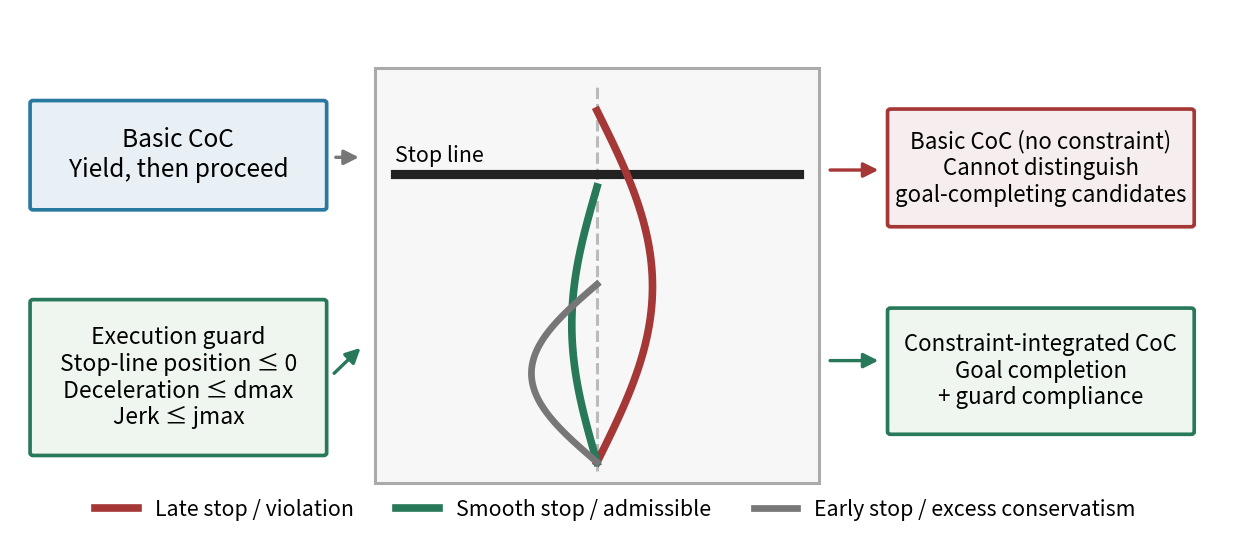
\includegraphics[width=0.98\textwidth]{../latex-kiee-review-2022/figures/fig01_concept.png}
\bifigcaption{기본 CoC와 제약 통합 CoC의 선택 기준 차이. 세 후보는 모두 `보행자에게 양보한 뒤 진행'이라는 목표와 관련되지만, 빨간 궤적은 정지선ㆍ동역학 제약을 위반하고 회색 궤적은 허용되지만 지나치게 보수적이다. 기본 CoC만으로는 두 실행 품질을 구별하기 어렵고, 제약 통합 CoC는 목표를 완료하면서 제약을 지키는 녹색 후보를 선택할 기준을 제공한다.}{Difference between basic CoC and constraint-integrated CoC: the latter distinguishes violating, overly conservative, and admissible goal-completing candidates.}
\label{fig:concept}
\end{figure*}

그림~\ref{fig:concept}은 동일한 "양보 후 진행" 목표를 달성하는 세 궤적 후보를 비교한다. 빨간색 궤적은 정지선이나 감속도ㆍ가가속도 제한을 위반하고, 회색 궤적은 필요 이상으로 일찍 정지하여 진행성을 잃는다. 반면 녹색 궤적은 행동 목표를 달성하면서 실행 가드도 만족한다. 요구사항만 포함한 CoC는 이 후보들을 명확히 구분하기 어렵지만, Safety-Constrained CoC는 목표를 유지하면서 허용 가능한 궤적을 선택할 기준을 제공한다.

제안한 가드가 궤적 선택에 실제로 영향을 주는지 확인하기 위해 같은 장면, 같은 행동 목표 및 같은 궤적 후보를 사용하되 실행 조건만 다른 두 문제를 한 쌍으로 구성한다. 이를 쌍대 계약(paired-contract) 벤치마크라 한다. 한 문제는 더 자유로운 행동을 허용하고 다른 문제는 실행 조건을 더 엄격하게 적용하므로, 두 문제에서 선택해야 할 궤적이 달라진다. 따라서 장면만 외운 모델은 두 문제를 모두 맞힐 수 없으며, 제시된 가드를 읽고 판단해야 한다. 정적 과제에서는 모든 후보가 기본 행동 목표를 달성하도록 구성하였다. 시간 과제에서는 서로 경쟁하는 진입 후보들이 목표를 달성하고, 계속 정지하는 후보는 낮은 위반률만을 노리는 교착 대조군으로 남겼다.

본 논문의 연구 질문은 다음과 같다.
\begin{enumerate}
    \item \textbf{RQ1 효과:} \sccoc{}는 요구사항만 포함한 CoC보다 가드를 위반하는 궤적의 선택을 줄이는가?
    \item \textbf{RQ2 목표 보존:} 가드 위반의 감소가 항상 정지하거나 교착되는 방식이 아니라, 행동 목표를 완료하면서 나타나는가?
    \item \textbf{RQ3 적용 범위:} 이러한 효과가 정적 후보 선택, 시간에 따른 유지ㆍ해제, 정지 및 차선 변경 상황에서도 반복되는가?
    \item \textbf{RQ4 입력 변화 강건성:} 동일 의미 문장 변형, 학습에 없던 수치, 부정ㆍ금지 표현, 경계 등호 및 단위 변환에서도 효과가 유지되는가?
\end{enumerate}

본 논문의 기여는 다음과 같다.
\begin{enumerate}
    \item 행동의 이유와 목표를 설명하는 CoC에 실행 가드를 결합한 \sccoc{}를 제안한다.
    \item 동일한 장면에서 실행 조건만 바꾸는 쌍대 계약 평가와, 행동 목표는 달성하지만 가드를 위반하는 반례 구성 방법을 제시한다.
    \item 가드 위반, 목표 완료, 교착, 과도한 보수성 및 계약 쌍의 정확도를 함께 측정하는 평가 체계를 구성한다.
    \item 한 난수 초기값(seed)의 정적 후보 실험과 데이터 생성 및 학습 난수를 함께 바꾼 세 난수 초기값의 시간ㆍ다중 주행 과제를 통해, 소형 VLM의 가드 기반 후보 선택이 표준 평가에서는 학습되지만 미관측 시간값 평가에서는 크게 약화됨을 함께 보인다.
    \item 저장한 세 난수 초기값의 어댑터를 원본ㆍ단색ㆍ충돌 영상에서 다시 평가하여, 표준 시간 과제는 영상에 의존하지만 다중 주행의 표준ㆍ미관측 수치 평가는 수치가 적힌 문장만으로 해결됨을 분리한다.
    \item 단일 장면 Alpamayo-R1 진단과 별도 소형 신경망 폐루프 실험을 보조 증거로 제시하여, 입력 문장에 대한 반응, 학습된 후보 선택 및 실행 중 강제 적용을 서로 구분한다.
\end{enumerate}

\revtwo{제안 방법의 장점은 네 가지다. 첫째, 기존 CoC의 설명 구조를 유지하면서 누락되기 쉬운 허용ㆍ금지ㆍ해제 조건을 자연어로 명시할 수 있다. 둘째, 쌍대 계약은 장면과 행동 목표를 고정하므로 높은 정확도가 장면 암기인지 가드에 따른 선택 전환인지 구분한다. 셋째, 가드 위반률과 목표 완료ㆍ교착ㆍ과도한 보수성을 함께 측정하여 항상 정지하는 해법을 성공으로 세지 않는다. 넷째, 후보 선택과 수치 판정을 분리하므로 같은 가드를 모델 외부 결정적 검증기 또는 실행 차단장치로 연결할 수 있다. 이 장점들은 합성 후보 선택의 해석 가능성과 진단 가능성에 관한 것이며 실제 차량의 안전 보장을 뜻하지 않는다.}

본 연구는 합성 이미지와 수치 설명으로 제시된 궤적 후보를 사용하여 소형 VLM의 학습 가능성을 평가한다. 영상 절제에서 표준 시간 과제는 여러 시점을 이어 붙인 연속 장면 영상에 의존했지만, 다중 주행의 표준ㆍ미관측 수치 평가는 단색 영상과 반대 행동 영상에서도 성능이 유지되어 문장 정보만으로 풀 수 있었다. 따라서 합성 영상의 시간 정보 사용은 확인했으나 실제 도로의 시각적 근거화를 입증하지는 않는다. 실험에 사용한 정지선, 최소 간격, 속도 및 대기시간 가드는 제안한 표현과 평가 방법을 시험하기 위해 연구자가 미리 정한 조건이다. 실제 도로의 CoC로부터 어떤 제약 조건을 선택하고 그 수치와 해제 조건을 어떻게 도출할 것인지도 본 논문에서 제시하거나 검증하지 않는다. 따라서 실제 차량의 충돌 감소, Alpamayo-R1을 학습한 뒤의 성능 향상 또는 완전한 도로 안전 명세를 입증하지는 않는다.

\revtwo{이후 논문의 흐름은 다음과 같다. 2장은 driving VLM과 실행 검증 연구 사이의 공백을 정리하고, 3장은 행동 목표와 실행 가드를 분리하여 선택 문제를 정의한다. 4장은 Safety-Constrained CoC 입력, 쌍대 계약 및 모델 외부 검증 지표를 제시한다. 5장은 정적ㆍ시간ㆍ다중 주행 후보 선택과 별도 폐루프 보조 실험을 순서대로 보고한다. 6장은 결과의 의미와 학습된 가드 준수ㆍ실제 실행 안전의 경계를 논의하고, 7장은 결론과 후속 과제를 정리한다.}

\section{관련 연구}
\label{sec:related}

\subsection{추론 보강형 E2E/VLA 자율주행}

DriveLM은 주행 장면을 그래프 기반 시각 질의응답으로 구조화하고 \cite{sima2024drivelm}, DriveVLM은 VLM의 장면 이해와 계획을 결합한다 \cite{tian2024drivevlm}. Alpamayo-R1은 CoC 추론과 행동/궤적 예측을 연결하여 긴 꼬리 상황에서의 일반화를 목표로 한다 \cite{wang2025alpamayo}. 한편 자율주행 VLM의 신뢰성 연구는 장면 이해와 행동 추론의 평가 지표 및 데이터 품질 문제를 지적한다 \cite{xie2025drivebench}. 본 연구는 객체 환각이나 CoC의 일반적 사실 오류를 다시 검출하기보다, 동일한 행동 목표를 달성하는 후보 안에서 명시된 허용조건을 학습하고 적용할 수 있는지를 다룬다.

\subsection{주행 안전 제약과 검증}

자율주행 안전 연구는 안전거리, 책임 민감 안전 모델, 도달 가능성, 실행시간 감시기(runtime monitor)와 차단장치(shield)처럼 실행 단계에서 제약을 검사하는 방법을 발전시켜 왔다 \cite{shalev2017rss,katz2019marabou}. 시나리오 명세 및 폐루프 시험은 보지 않은 조합에서 학습 정책의 취약성을 발견하는 데 사용된다 \cite{fremont2019scenic,zhang2023cat}. 이러한 방법은 정밀한 제약 집행에 적합하지만 자연어 추론과 실행 계약 사이의 인터페이스는 별도 문제다.

\subsection{자연어와 정형 명세의 역할}

자연어는 사전학습 VLM이 처리하기 쉬우며 사람에게 편리하지만, 부정 범위, 단위 및 경계 연산자가 모호할 수 있다. 정형 명세는 정확한 판정과 실행 단계의 강제 적용에 적합하지만 기반 VLM이 임의 논리 문법을 즉시 실행할 것이라고 가정할 수 없다. 본 논문은 두 표현을 경쟁 관계로 두지 않는다. 자연어 \sccoc{}를 학습 인터페이스로 평가하고, 수치 판정은 모델 외부의 결정적 검증기로 계산한다. 자연어에서 구조화 계약(typed contract)으로의 변환은 후속 연구로 남긴다.

\subsection{차별점}

본 연구는 실제 사고 궤적을 필요로 하지 않는다. 정적 과제에서는 모든 후보가 CoC 목표를 달성하되 가드 준수 여부와 진행도가 다르게 구성하고, 시간 과제에서는 계속 정지하는 교착 대조군을 추가한다. 또한 동일 장면의 계약만 바꾸는 쌍대 계약과 제약--정답 대응 교란 통제군을 사용하여 위반 감소와 목표 완료를 함께 평가한다.

\revtwo{표~\ref{tab:prior-comparison}은 연구 공백과 본 연구의 위치를 요약한다. 기존 driving VLM/CoC의 중심은 장면 이해와 행동 근거를 포함한 계획이고, 형식 실행 검증의 중심은 이미 주어진 명세의 정확한 판정과 강제 적용이다. 본 연구는 두 흐름의 성능을 대체하거나 직접 비교하지 않는다. 자연어 가드를 CoC 학습 입력에 포함하고, 동일 장면의 가드만 바꾸는 반사실적 평가와 모델 외부 수치 판정을 연결하는 중간 인터페이스를 제안한다.}

\begin{table*}[!t]
\color{reviewertwo}
\centering
\bitablecaption{관련 연구 흐름과 본 연구의 역할 비교. 이 표는 성능 순위가 아니라 연구 질문과 증거 범위의 차이를 나타낸다.}{Comparison of research roles and evidence scopes; the rows are not a performance ranking.}
\label{tab:prior-comparison}
\scriptsize
\begin{tabularx}{\textwidth}{YYYYY}
\toprule
Research line & Primary role & Execution condition & Diagnostic evaluation & Evidence scope \\
\midrule
Driving VLM / CoC & Explain scene causes and predict actions or trajectories & May remain implicit in the behavioral objective & Scene and planning benchmarks & Learned reasoning and planning \\
Formal monitor / shield & Check or override an executed command & Explicit formal rule supplied to the monitor & Rule satisfaction during execution & Enforcement under the supplied specification \\
Safety-Constrained CoC (ours) & Select a goal-completing candidate under an added guard & Natural-language guard coupled to the CoC; candidate values checked deterministically & Fixed-scene guard swap, shuffled mapping, violation and completion metrics & Guard-based synthetic candidate selection; no vehicle-safety guarantee \\
\bottomrule
\end{tabularx}
\end{table*}

\section{문제 정의}
\label{sec:problem}

\revtwo{앞 절에서 확인한 연구 공백을 선택 문제로 구체화한다. 핵심은 행동 목표를 달성했는지와 그 행동이 현재 실행 가드 안에서 허용되는지를 서로 다른 판정으로 두는 것이다. 이 구분을 먼저 정의한 뒤, 다음 장에서 모델 입력과 쌍대 계약 평가로 구현한다.}

장면 입력을 $x$, 요구사항을 기술한 CoC를 $R$, 실행 가드를 $G$, 궤적 후보 집합을 $\mathcal{T}(x)=\{\tau_1,\ldots,\tau_K\}$라 하자. $\mathrm{Goal}(\tau,R)$는 후보가 요구사항의 행동 목표를 완료하는지, $\mathrm{Sat}(\tau,G)$는 후보가 실행 가드를 만족하는지를 나타낸다. 궤적의 진행도 또는 효용은 $U(\tau)$로 둔다. 본 연구의 선택 목표는 다음과 같다.
\begin{equation}
\begin{aligned}
\tau^*&=\arg\max_{\tau\in\mathcal{T}(x)} U(\tau),\\
\mathrm{s.t.}\quad &\mathrm{Goal}(\tau,R)=1,\quad \mathrm{Sat}(\tau,G)=1.
\end{aligned}
\label{eq:selection}
\end{equation}

$\mathrm{Goal}=1$이지만 $\mathrm{Sat}=0$인 후보는 행동 목표를 달성하더라도 현재 실행 조건을 위반하는 반례다. 반대로 가드를 위반하지 않지만 목표를 완료하지 못하는 후보는 교착 후보로 구분한다. 따라서 항상 정지하는 정책은 가드 위반률이 낮더라도 바람직한 정책으로 볼 수 없다.

\begin{table}[t]
\centering
\bitablecaption{실행 가드를 구성하는 일곱 요소. 각 행은 `언제 의무가 시작되는가, 유지 중 무엇을 지켜야 하는가, 언제 끝나는가, 불확실하면 무엇을 하는가' 중 하나를 담당한다. 모든 장면에 일곱 요소를 전부 쓰는 것은 아니다.}{Seven compositional elements of an execution guard; only elements relevant to a scene and objective are selected.}
\label{tab:taxonomy}
\footnotesize
\begin{tabularx}{\columnwidth}{L{0.30\columnwidth}Y}
\toprule
Type & Meaning and example \\
\midrule
Activation & Activate the yielding obligation when a pedestrian enters the conflict zone \\
Invariant & Do not cross the stop line while the obligation is active \\
Bound & Vehicle gap $\geq6$ m; deceleration $\leq4$ m/s$^2$ \\
Prohibition & Do not continue a lane change while the vehicle gap is below the threshold \\
Release & Permit departure after the conflict zone remains clear for 1.5 s \\
Fallback & Remain stopped when the observation is uncertain \\
Termination & Complete the lane change while maintaining a safe gap \\
\bottomrule
\end{tabularx}
\end{table}

\subsection{표 1로부터 S-C CoC 구성}

표~\ref{tab:taxonomy}는 하나의 완성된 안전 명세가 아니라 장면과 행동 목표에 따라 선택하는 실행 가드의 구성 요소를 제시한다. 표에 정리된 일곱 가지 가드 유형의 집합을 $\mathcal{G}_{\mathrm{tax}}$라 하고, 장면 $x$와 요구사항 $R$에 필요한 가드의 부분집합을 $\mathcal{S}(x,R)$라 하면, 실행 가드와 S-C CoC의 구성 관계는 다음과 같이 나타낼 수 있다.
\begin{equation}
\begin{aligned}
\mathcal{S}(x,R)&\subseteq\mathcal{G}_{\mathrm{tax}},\\
G(x,R)&=\bigwedge_{g\in\mathcal{S}(x,R)}g,\\
\mathrm{SCCoC}(x,R)&=R\oplus G(x,R).
\end{aligned}
\label{eq:sccoc-compose}
\end{equation}
여기서 $\oplus$는 행동 요구사항과 선택된 가드 문장을 하나의 S-C CoC로 결합함을 뜻한다. 표의 모든 유형을 항상 사용하는 것은 아니며, 장면과 목표에 관련된 조건만 선택한다.

\paragraph{보행자 양보 예.}
기본 CoC가 "보행자에게 양보한 뒤 진행한다"라면 활성화, 불변 조건, 수치 경계, 해제 조건 및 대체 동작을 선택할 수 있다. 이때 표~\ref{tab:taxonomy}로부터 다음 S-C CoC를 구성할 수 있다.
\begin{quote}
\small
보행자가 상충 구역에 있으면 양보 의무를 활성화한다. 의무가 활성화된 동안 정지선을 넘지 않고 감속도를 $4\,\mathrm{m/s^2}$ 이하로 유지한다. 관측이 불확실하면 정지 상태를 유지한다. 상충 구역이 1.5초 이상 연속으로 비어 있을 때만 의무를 해제하고 출발한다.
\end{quote}
이 문장은 단순히 "양보한다"는 목표뿐 아니라 정지 위치, 감속 한계, 불확실할 때의 행동 및 출발 허용 시점을 함께 규정한다.

\paragraph{차선 변경 예.}
기본 CoC가 "안전하게 목표 차선으로 이동한다"라면 수치 경계, 금지 조건, 해제 조건 및 종료 조건을 선택할 수 있다. 구성된 S-C CoC는 다음과 같다.
\begin{quote}
\small
목표 차선의 차량 간격이 6 m 미만이면 차선 변경을 계속하지 않는다. 안전 간격이 다시 확보되면 차선 변경을 재개할 수 있다. 목표 차선에 진입한 뒤 안전 간격이 유지될 때 차선 변경을 완료한다.
\end{quote}
이 예에서는 같은 차선 변경 목표라도 차량 간격에 따라 계속 진행, 중단, 재개 및 완료 시점이 달라진다.

표~\ref{tab:taxonomy}만으로 장면에 필요한 S-C CoC가 자동으로 결정되는 것은 아니다. 장면에서 관측 가능한 상태와 기본 CoC의 행동 목표를 함께 사용하여 관련 가드를 선택해야 한다. 따라서 본 연구의 가드는 현재 데이터와 궤적 후보에서 측정 가능한 실행 의무를 구조화한 부분 계약이며, 완전한 도로 안전 명세를 의미하지 않는다.

\raggedbottom
\section{Safety-Constrained CoC와 평가 방법}
\label{sec:method}

본 장의 목적은 모델이 실행 가드를 실제로 읽고 궤적 선택에 사용하는지 확인하는 방법을 설명하는 것이다. 이를 분명하게 측정하기 위해 모델이 새로운 궤적을 직접 만들게 하지 않고, 미리 만든 여러 후보 중 하나를 고르게 한다. 모델이 직접 궤적을 만들면 궤적 생성 능력과 가드 이해 능력이 결과에 함께 섞인다. 후보 선택 문제로 범위를 좁히면, 같은 후보를 놓고 가드가 바뀔 때 모델의 선택도 바뀌는지를 직접 확인할 수 있다.

\revtwo{3장의 최적화 정의를 실제 평가 절차로 옮기기 위해 이 장은 세 질문에 순서대로 답한다. 모델에 무엇을 입력하는가, 가드 사용 여부를 어떤 대조군과 쌍대 계약으로 분리하는가, 그리고 선택 결과를 모델과 독립된 규칙으로 어떻게 판정하는가이다. 따라서 제안 방법의 출력은 연속 제어 명령이 아니라 후보 식별자이며, 검증기는 그 후보의 저장 측정값을 계약 경계와 비교한다.}

\subsection{제안 방법의 전체 흐름}

그림~\ref{fig:pipeline}의 과정은 세 단계로 이루어진다. 첫째, 모델에 장면 이미지, 기본 CoC, 실행 가드와 궤적 후보를 준다. 기본 CoC는 "보행자에게 양보한 뒤 진행한다"처럼 달성할 행동을 말한다. 실행 가드는 "정지선을 넘지 않는다" 또는 "차량이나 보행자의 이동 경로가 겹치는 구역이 1.5초 동안 비어 있을 때만 출발한다"처럼 그 행동을 언제, 어느 범위에서 허용할지를 정한다. 각 후보에는 정지 위치, 속도, 감속도, 가가속도(가속도가 변하는 정도), 차량 간격과 진입 시점이 함께 적혀 있다.

둘째, 모델은 이미지와 문장을 읽고 후보 하나를 선택한다. 셋째, 모델 외부의 결정적 검증기(verifier)가 선택된 후보의 수치를 다시 계산한다. 예를 들어 정지선을 넘었는지, 최소 간격을 지켰는지, 필요한 시간만큼 기다렸는지를 확인한다. 따라서 모델이 스스로 "안전하다"고 답한 것만으로 정답으로 인정하지 않는다. 모델의 선택과 검증기의 계산 결과가 모두 맞아야 가드를 지킨 선택으로 판정한다. 다만 후보 수치, 정답 생성 규칙과 검증 규칙은 같은 합성 과제 정의에서 만들어졌으므로, 이 검증기는 모델과는 분리되어 있지만 계약 자체의 타당성을 확인하는 외부 안전 정답은 아니다.

\begin{figure*}[!t]
\centering
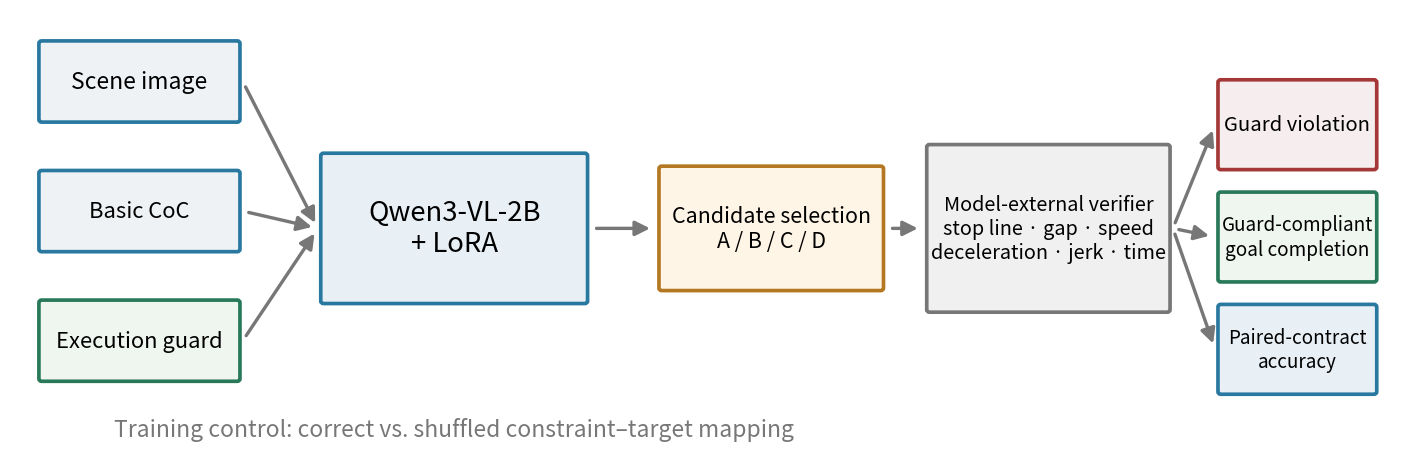
\includegraphics[width=0.98\textwidth]{../latex-kiee-review-2022/figures/fig02_pipeline.png}
\bifigcaption{제안 평가의 흐름. 왼쪽의 장면ㆍ기본 CoCㆍ실행 가드를 모델에 입력하면 모델이 가운데의 후보 A--D 중 하나를 선택한다. 오른쪽의 규칙 기반 검증기는 선택된 후보의 정지 위치, 간격, 속도 및 시간을 가드의 기준값과 비교하여 가드 위반률, 가드 준수 목표 완료율 및 계약 쌍 정확도를 계산한다. 검증기는 모델의 자기평가가 아니라 후보 수치에 결정 규칙을 적용한다.}{Evaluation pipeline from scene, basic CoC, and execution guard through candidate selection to model-external deterministic metric computation.}
\label{fig:pipeline}
\end{figure*}

\subsection{CoC와 실행 가드의 입력 방식}

본 연구는 기본 CoC에 실행 가드를 결합한 형식을 제안한다. 예를 들어 기본 CoC가 "횡단보도 앞 보행자에게 양보한 뒤, 허용되면 진행한다"라면 다음 조건을 덧붙일 수 있다.

\begin{quote}\small
정지선을 넘지 않는다. 최대 감속도는 $3.8\,\mathrm{m/s^2}$, 최대 가가속도는 $5.0\,\mathrm{m/s^3}$를 넘지 않는다. 상충 구역이 정해진 시간 동안 비어 있을 때만 출발한다.
\end{quote}

이 실행 가드를 기본 CoC 뒤에 이어서 한 문장 묶음으로 제시한 방식을 \textbf{제약 통합 CoC}라 한다. 이것이 본 논문의 Safety-Constrained CoC를 실험에 구현한 제안 조건이다. 모델은 이 입력에서 "무엇을 해야 하는가"와 "그 행동을 언제 허용하는가"를 함께 읽는다. 다만 성능이 좋아지더라도 그 이유가 가드의 의미를 배웠기 때문인지, 단순히 문장이 더 길어졌기 때문인지 구분해야 한다. 이를 위해 표~\ref{tab:representations}의 다섯 조건을 비교한다. 표와 그림 내부는 영어로 통일하여 각각 \textit{Basic CoC (no constraint)}, \textit{Constraint-integrated CoC (proposed)}, \textit{Separate natural-language constraint}, \textit{Shuffled constraint--target mapping}, \textit{Logical-form constraint}로 표시한다.

\begin{table*}[!t]
\centering
\bitablecaption{실험 조건의 공통 이름과 차이. `제약 통합 CoC'는 제안 조건이며, `제약--정답 대응 교란'은 제약 문장의 추가 효과와 올바른 의미 대응의 효과를 구분하기 위한 음성 통제군이다.}{Common names and differences among input conditions. The shuffled constraint--target condition is a negative control.}
\label{tab:representations}
\footnotesize
\begin{tabularx}{\textwidth}{L{0.19\textwidth}L{0.25\textwidth}Y}
\toprule
Condition & Model input & Purpose \\
\midrule
Basic CoC (no constraint) & Basic CoC describing only the behavioral objective & Information-absent baseline that cannot distinguish the two contracts \\
Constraint-integrated CoC (proposed) & Natural-language execution guard appended directly to the basic CoC & Learn the objective and admissibility conditions in one context \\
Separate natural-language constraint & The same natural-language guard supplied in a separate input field & \revone{Position-only ablation: preserve guard wording, examples, and training budget while changing its placement} \\
Shuffled constraint--target mapping & A constraint is supplied, but training pairs it with another example's target & Test whether correct constraint--action correspondence is necessary \\
Logical-form constraint & The same execution condition written in a fixed logical form & Test whether the current model handles a structured non-natural-language form \\
\bottomrule
\end{tabularx}
\end{table*}

특히 \textbf{제약--정답 대응 교란}은 음성 통제군이지 제안 방법이 아니다. 이 조건에도 동일한 제약 문장 집합이 들어가지만, 학습할 때 다른 예의 제약 문장을 옮겨 제약과 정답 후보의 연결을 깨뜨린다. 평가는 다시 올바른 제약으로 수행한다. 따라서 올바른 대응을 학습한 조건만 높은 성능을 보인다면, 단순히 문장이 길어지거나 제약 관련 단어가 들어간 효과로 설명하기 어렵다.

\revone{시간 과제에서는 두 개의 통제된 대비를 분리한다. 첫째, 제약 통합 CoC와 별도 자연어 제약은 동일한 가드 문장, 장면, 후보, 정답, 384개 학습 예, 3 epoch 및 최적화 설정을 사용한다. 차이는 가드를 기본 CoC 문장 뒤에 이어 붙이는지, 동일 문장을 별도 \texttt{Temporal safety guard} 필드에 두는지뿐이므로 이 비교는 위치ㆍ구획 형식의 효과를 측정하는 position-only ablation이다. 둘째, 별도 자연어 제약과 제약--정답 대응 교란은 입력 위치를 같게 유지하고 학습 시 가드와 정답의 대응만 깨뜨리므로 올바른 의미 대응의 필요성을 측정한다. 이 두 대비는 위치 효과와 대응 효과를 구분하지만, 시간 과제에 통합 위치의 대응 교란 조건이 없으므로 완전한 $2\times2$ 요인 설계는 아니다. 따라서 제약 통합 CoC와 대응 교란의 전체 차이를 의미 학습만의 효과로 해석하지 않는다. 다중 주행 과제에서는 제약 통합 CoC와 대응 교란이 같은 형식이다. \textbf{논리식 제약}도 자연어와 논리식 중 어느 쪽이 본질적으로 우수한지 판정하기 위한 조건이 아니라, 현재 VLM과 학습 방법이 두 표현을 얼마나 잘 처리하는지 확인하기 위한 조건이다.}

\subsection{같은 장면에서 실행 조건만 바꾸는 평가}

한 장면으로 정답이 서로 다른 두 문제를 만든다. 두 문제에는 같은 이미지, 같은 CoC 목표와 같은 궤적 후보를 사용한다. 바꾸는 것은 실행 가드뿐이다. 가드가 달라지면 올바른 후보도 달라지게 구성한다. 따라서 모델이 두 문제를 모두 맞히려면 장면만 보고 같은 답을 반복해서는 안 되고, 가드를 읽은 뒤 선택을 바꾸어야 한다. 이 두 문제의 묶음을 \textbf{쌍대 계약(paired-contract)}이라 한다.

그림~\ref{fig:pair}은 차선 변경 예에서 무엇이 고정되고 무엇이 바뀌는지를 보여준다. 두 계약 모두 현재 차량 간격은 7.2 m이며 후보도 같다. 후보 A는 현재 간격에서 바로 차선을 변경하고, 후보 B는 차선 변경을 중단한 뒤 필요한 간격이 확보되면 다시 시도한다. 최소 간격이 5.5 m인 완화 계약에서는 $7.2 \geq 5.5$이므로 후보 A가 허용되고 진행도가 높은 후보 A를 선택한다. 반면 최소 간격이 9.0 m인 엄격 계약에서는 $7.2 < 9.0$이므로 후보 A가 가드를 위반하고 후보 B를 선택해야 한다.

즉, 완화 계약과 엄격 계약은 장면이 아니라 허용 기준만 다르다. 모델이 두 문제에 같은 후보를 답하면 적어도 하나는 틀린다. "계약 쌍 정확도"는 두 문제를 모두 맞혔을 때만 그 쌍을 정답으로 계산한다. 이 값이 높을수록 모델이 최소 간격의 변화를 읽고 선택에 반영했다고 볼 수 있다.

\begin{figure*}[!t]
\centering
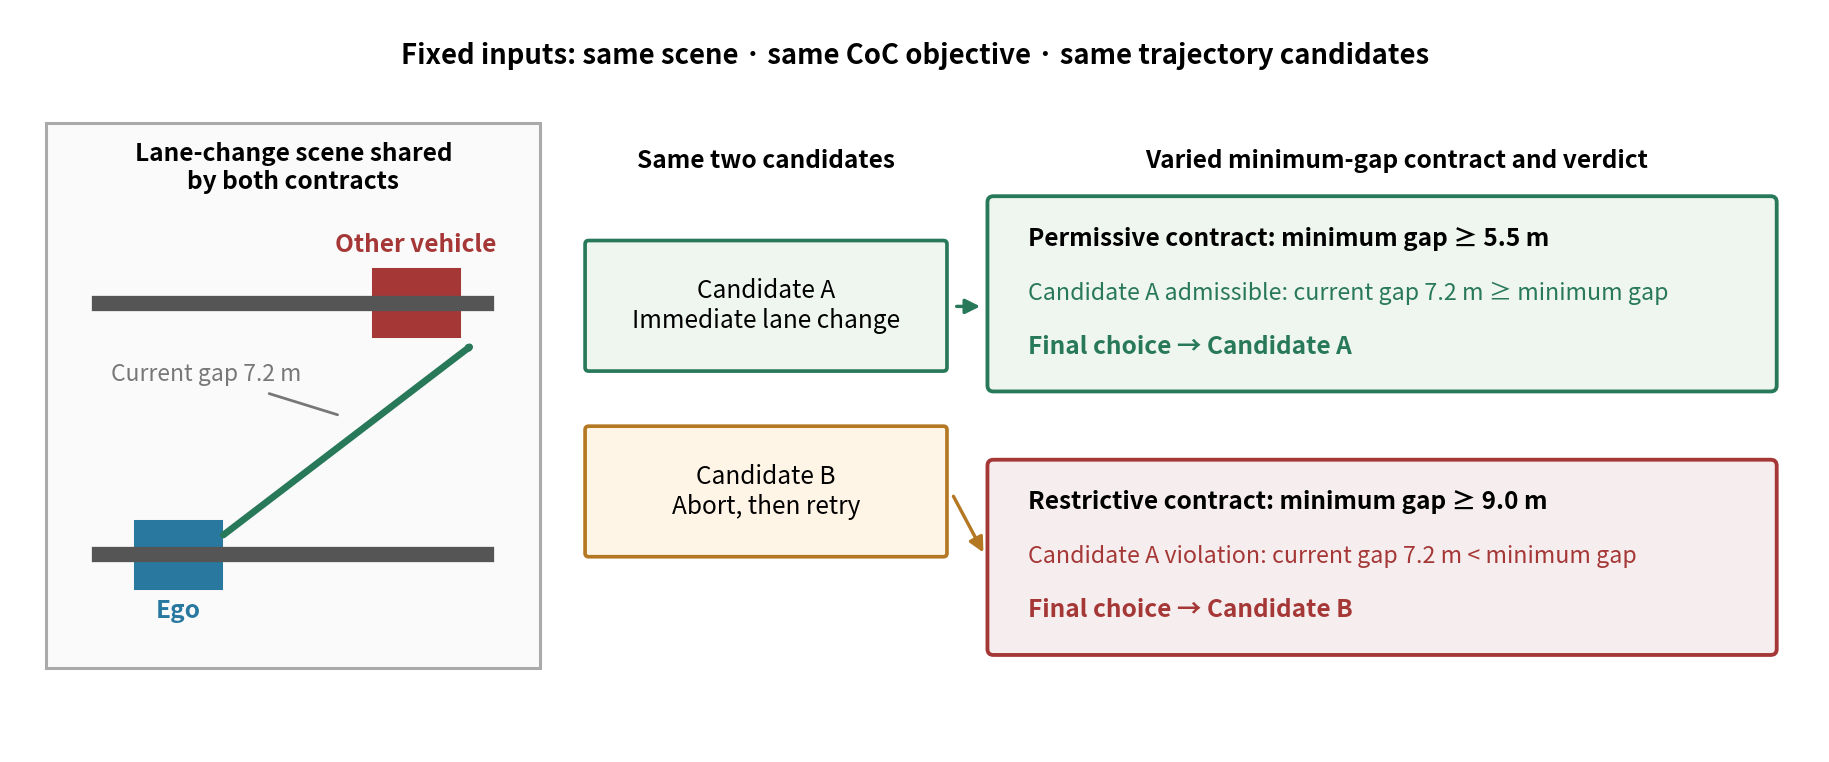
\includegraphics[width=0.98\textwidth]{../latex-kiee-review-2022/figures/fig03_paired_contract.png}
\bifigcaption{쌍대 계약의 차선 변경 예. 장면, CoC 목표, 현재 간격 7.2 m 및 후보 A/B는 고정하고 최소 간격만 5.5 m에서 9.0 m로 바꾼다. 완화 계약에서는 즉시 차선 변경하는 후보 A가 허용되지만, 엄격 계약에서는 같은 후보가 최소 간격을 위반하므로 중단 후 재시도하는 후보 B를 선택한다.}{Paired-contract lane-change example with fixed scene, objective, current gap, and candidates but different minimum-gap contracts.}
\label{fig:pair}
\end{figure*}

시간 과제에서는 행동이 다른 네 후보를 사용한다. 모델은 $A$, $B$, $C$, $D$ 중 하나를 답하지만, 이 문자는 후보를 구별하기 위한 이름일 뿐이다. 예를 들어 $A$가 언제나 조기 진입을 뜻하는 것은 아니다. 표~\ref{tab:candidate-roles}은 후보가 실제로 수행하는 네 가지 행동을 보여준다.

\begin{table*}[!t]
\centering
\bitablecaption{시간 과제 후보를 행동 의미로 해석하는 방법. 행은 후보 문자가 아니라 실제 행동 역할이며, 열은 같은 장면에 적용한 짧은 대기(완화)와 긴 대기(엄격) 계약의 판정이다. 완화 계약은 짧은 대기 후 진입, 엄격 계약은 긴 대기 후 진입을 정답으로 만든다.}{Behavioral roles of temporal candidates under short-wait permissive and long-wait restrictive contracts.}
\label{tab:candidate-roles}
\footnotesize
\begin{tabularx}{\textwidth}{L{0.18\textwidth}L{0.29\textwidth}L{0.20\textwidth}Y}
\toprule
Trajectory role & Behavior & Permissive contract & Restrictive contract \\
\midrule
Early entry & Enter before the conflict zone becomes clear & Guard violation & Guard violation \\
Entry after a short hold & Proceed after a short clear-zone hold & Preferred admissible candidate & Violation: insufficient hold time \\
Entry after a long hold & Proceed after a longer confirmation interval & Admissible but less progress & Preferred goal-completing candidate \\
Remain stopped & Stay stopped until the evaluation ends & Goal incomplete or deadlock & Goal incomplete or deadlock \\
\bottomrule
\end{tabularx}
\end{table*}

한 장면에서는 $A$가 조기 진입이고 $B$가 짧은 대기일 수 있다. 다음 장면에서는 문자와 행동의 대응을 바꾸어 $A$가 긴 대기를 나타내게 할 수 있다. 이렇게 하면 모델이 항상 같은 문자만 고르는 방법으로 정답을 외울 수 없다. 정적 실험은 두 후보 $A/B$를, 시간 및 다중 주행 실험은 네 후보 $A/B/C/D$를 사용한다. 어느 실험에서도 특정 문자가 항상 안전하거나 항상 위험한 행동을 뜻하지 않는다.

\subsection{모델 학습과 정답 후보 생성}

기반 모델은 Qwen3-VL-2B-Instruct이다. 전체 모델을 다시 학습하지 않고 일부 추가 매개변수만 조정하는 LoRA 방식을 사용한다. 모델이 한 번에 받는 학습 자료는 다음 다섯 부분으로 구성된다.

\begin{enumerate}
\item 장면을 나타내는 합성 이미지,
\item 달성해야 할 행동을 설명하는 기본 CoC,
\item 실험 조건에 따른 실행 가드,
\item 각 후보의 행동과 측정값을 적은 설명,
\item 허용되는 후보 중 진행도가 가장 높은 후보를 고르라는 지시.
\end{enumerate}

모델은 후보 문자 하나를 답한다. 정답은 다음 세 단계로 정한다. 먼저 CoC의 행동 목표를 끝내지 못한 후보를 제외한다. 그다음 실행 가드를 위반한 후보를 제외한다. 마지막으로 남은 후보 중에서 가장 원활하게 진행하는 후보를 정답으로 삼는다. 모든 장면에는 목표와 가드를 함께 만족하는 후보가 적어도 하나 있다. 이는 식~\eqref{eq:selection}을 학습 자료 생성에 그대로 적용한 것이다.

예를 들어 가장 빨리 진행하는 후보가 최소 간격을 위반하면 정답이 될 수 없다. 반대로 가드 위반을 피하기 위해 끝까지 정지하는 후보도 행동 목표를 완료하지 못하므로 정답이 아니다. 모델은 "진행"과 "가드 준수"를 동시에 만족하는 후보를 찾아야 한다.

\subsection{모델 외부 궤적 검증과 평가 지표}

모델의 답은 $A$와 같은 후보 문자일 뿐이다. 이 답이 실제로 가드를 지켰는지는 별도 검증기가 계산한다. 검증기는 표~\ref{tab:verifier-fields}의 수치를 후보 데이터에서 읽고 가드의 기준과 직접 비교한다. 예를 들어 최소 간격이 9.0 m라면 선택한 후보의 간격이 9.0 m 이상인지 확인한다.

\begin{table}[t]
\centering
\bitablecaption{모델 외부 검증기의 판정값과 읽는 법. 검증기는 모델의 설명을 믿지 않고 선택된 후보의 저장 수치를 계약 경계와 직접 비교한다.}{Values used by the model-external deterministic verifier, which compares stored candidate measurements directly with contract bounds.}
\label{tab:verifier-fields}
\footnotesize
\begin{tabularx}{\columnwidth}{L{0.34\columnwidth}Y}
\toprule
Checked value & Example decision \\
\midrule
Stop-line-relative position & Crossing is detected when the position exceeds 0 m \\
Maximum speed & Check whether the allowed speed limit is exceeded \\
Maximum deceleration & Check whether the hard-braking limit is exceeded \\
Maximum jerk & Check whether the acceleration-change limit is exceeded \\
Minimum vehicle gap & Check whether the required distance to another vehicle is maintained \\
Intersection entry time & Check the required hold after the conflict zone becomes clear \\
\bottomrule
\end{tabularx}
\end{table}

표~\ref{tab:method-metrics}은 평가에 사용한 지표를 정리한다. 비율의 분모는 별도 표기가 없으면 해당 평가의 전체 예다. 이 가운데 "가드 준수 목표 완료율"은 두 가지를 동시에 만족한 비율이다. 첫째, 선택한 후보가 CoC의 행동 목표를 완료해야 한다. 둘째, 실험에서 제시한 실행 가드를 모두 지켜야 한다. 이 지표는 실제 도로의 모든 위험이 제거되었다는 뜻은 아니다.

\begin{table}[t]
\centering
\bitablecaption{표와 그림에 반복해서 사용하는 지표. 후보 정확도ㆍ가드 준수 목표 완료율ㆍ계약 쌍 정확도는 높을수록 좋고, 가드 위반률ㆍ교착률ㆍ과도한 보수 선택률은 낮을수록 좋다.}{Metrics used throughout the tables and figures, including their preferred directions.}
\label{tab:method-metrics}
\footnotesize
\begin{tabularx}{\columnwidth}{L{0.31\columnwidth}Y}
\toprule
Metric & Meaning \\
\midrule
Candidate accuracy & Fraction selecting the optimal candidate defined by the data-generation rule \\
Guard violation rate & Fraction whose selected candidate violates at least one execution guard \\
Guard-compliant goal completion rate & Fraction that both satisfies the guard and completes the basic-CoC objective \\
Deadlock rate & Fraction that avoids violation but remains stopped without completing the objective \\
Excess-conservatism rate & Fraction selecting an unnecessarily slow candidate when a more progressive admissible one exists \\
Paired-contract accuracy & Fraction of scene pairs for which both permissive and restrictive contracts are answered correctly \\
\bottomrule
\end{tabularx}
\end{table}

\revtwo{모델 외부 검증을 사용하는 이유는 모델의 설명이나 자기평가와 실제 수치 판정을 분리하기 위해서다. Candidate accuracy는 생성 규칙이 정한 최적 후보와의 일치를, guard violation rate는 선택 후보가 명시된 경계를 넘었는지를, guard-compliant goal completion은 준수와 목표 달성을 동시에 측정한다. Deadlock과 excess-conservatism은 위반률만 낮추기 위한 정지 또는 불필요한 감속을 드러낸다. Paired-contract accuracy는 같은 장면에서 가드가 바뀔 때 두 선택을 모두 맞혔는지를 측정한다. 따라서 한 지표의 높은 값만으로 성공을 선언하지 않고, 외부 검증 결과와 상호 보완적인 지표를 함께 사용한다.}

\revone{평가 장면 쌍이 $N$개이면 후보 정확도는 $2N$개의 개별 계약 문제 중 맞힌 비율이고, 계약 쌍 정확도는 $N$개 장면 중 완화ㆍ엄격 계약을 모두 맞힌 비율이다. 예를 들어 두 장면 쌍에서 첫 쌍의 두 계약과 둘째 쌍의 완화 계약만 맞히면 후보 정확도는 $3/4=0.75$이지만 계약 쌍 정확도는 $1/2=0.50$이다. 두 계약에 항상 같은 후보를 답하는 모델은 각 쌍에서 한 문제를 맞혀 후보 정확도 0.50을 얻을 수 있지만, 계약에 따라 선택을 전환하지 못하므로 계약 쌍 정확도는 0이다. 따라서 계약 쌍 정확도는 단순히 더 어려운 정확도가 아니라, 동일한 장면ㆍ목표ㆍ후보에서 가드 변화에 맞추어 두 선택을 모두 올바르게 전환하는 능력을 추가로 측정한다.}

\subsection{학습된 가드 준수와 실제 실행 안전의 구분}

본 연구가 확인하는 것은 모델이 주어진 후보 중에서 가드를 지키는 후보를 더 잘 고를 수 있는가이다. 이것은 실제 차량에서 충돌을 막는 안전 보장과 다르다. 여기서 사용한 검증기는 합성 과제의 규칙으로 실험 결과를 계산하는 도구이며, 차량의 명령을 실시간으로 막거나 수정하는 차단 장치가 아니다.

\revtwo{두 개념을 구분하는 이유는 평가 단위와 고려하는 실패 원인이 다르기 때문이다. 학습된 가드 준수는 유한한 합성 후보와 연구자가 제공한 부분 계약 안에서 $\mathrm{Goal}$과 $\mathrm{Sat}$를 만족하는 선택의 비율이다. 실제 실행 안전은 센서 오인식, 계약에 빠진 위험, 연속 궤적 오차, 차량 동역학, 다른 도로 사용자의 반응 및 지연된 상태 갱신까지 포함하는 폐루프 성질이다. 따라서 후보 평가에서 준수율이 1.000이더라도 가드가 불완전하거나 관측이 틀리면 실제 차량은 위험할 수 있다. 이 구분은 높은 합성 점수를 안전 보장으로 확대하는 범주 오류를 막고, 최신 상태를 사용하는 외부 검증기와 차단장치가 별도로 필요한 이유를 드러낸다.}

실제 차량에 적용하려면 두 단계가 더 필요하다. 먼저 자연어 가드에서 조건의 종류, 비교 방향, 수치, 단위와 조건을 지킬 수 없을 때의 대체 행동을 정확히 추출해야 한다. 예를 들어 "최소 간격 9 m"를 "거리, 이상, 9, m"처럼 일정한 형식으로 바꾸고 단위도 통일해야 한다. 다음으로 모델이 만든 궤적을 출처가 추적되는 안전 요구사항에 연결된 외부 검증기나 실행 차단 장치가 다시 검사해야 한다. 따라서 본 연구는 제한된 후보 선택 과제에서 가드 준수를 학습할 수 있음을 보일 뿐, 실제 도로의 완전한 안전 명세나 차량 안전을 보장하지 않는다.

\section{실험 및 결과}
\label{sec:experiments}

\revtwo{4장에서 정의한 입력ㆍ대조군ㆍ외부 검증 지표를 단계적으로 적용한다. 먼저 추가 학습 없이 가드 문장에 반응하는지를 진단하고, 이어 올바른 가드--행동 대응의 학습 가능성을 확인한다. 그다음 동일 목표의 정적 후보, 시간 유지ㆍ해제, 정지ㆍ차선 변경으로 적용 범위를 넓히고, 마지막에 별도 폐루프 환경에서 실행 차단의 역할을 분석한다. 각 실험은 확인 목적, 비교 방법, 결과 및 의미의 순서로 기술한다.}

실험 증거는 서로 직접 비교할 수 없는 세 묶음으로 나뉜다. 첫째, 추가 학습을 하지 않은 Alpamayo-R1의 단일 장면 사전 진단은 가드 문장에 대한 반응만 살펴본다. 둘째, 본 논문의 중심 증거인 Qwen3-VL-2B-Instruct 실험은 합성 정적ㆍ시간ㆍ다중 주행 과제에서 가드 기반 후보 선택의 학습 가능성을 평가한다. 셋째, 별도의 두 층 신경망과 1차원 운동 모델을 이용한 폐루프 실험은 실행 차단장치의 역할을 분석하는 보조 증거다. 서로 다른 모델과 과제를 하나의 성능 향상 계열이나 교차 모델 재현으로 해석하지 않는다.

Qwen 실험은 단순한 정지/진행 문제에서 시작한다. 이 과제는 장면만 보고도 답을 맞힐 수 있다는 한계가 있으므로, 이후에는 같은 장면과 같은 행동 목표를 유지하고 가드만 바꾸어 정답이 달라지는 쌍대 계약을 사용한다. 평가 범위는 정적 경계, 대기와 출발의 시간 조건, 정지와 차선 변경 순으로 넓힌다.

이 장에서 사용하는 "가드 준수 목표 완료율"은 실험에서 제시한 가드를 지키면서 CoC의 행동 목표까지 끝낸 예의 비율이다. 실제 도로의 모든 위험이 제거되었다는 뜻은 아니다. \revone{서로 다른 설정과 지표를 사용하는 실험의 역할을 먼저 구분할 수 있도록, 표~\ref{tab:suite}에 각 실험의 연구 질문ㆍ평가 설정, 핵심 비교, 주요 지표 및 증거의 범위를 함께 정리하였다. 행 사이의 절대 수치는 비교하지 않고 각 행의 핵심 비교 안에서 해석한다.}

\paragraph{평가 이름을 읽는 법.}
이후 모든 과제에서 \textbf{표준 평가}는 학습에 쓰지 않은 장면을 사용하되 문장 틀과 수치 범위는 학습 자료와 같은 평가를 뜻한다. \textbf{동일 의미 문장 변형 평가}는 제약의 뜻과 수치는 유지하고 문장 표현만 바꾼다. \textbf{미관측 수치 평가}는 문장 틀은 유지하되 학습에 없던 속도ㆍ거리ㆍ시간 값을 사용하며, 시간 과제에서는 이를 \textbf{미관측 시간값 평가}라 부른다. \textbf{복합 표현 변화 평가}는 경계값 등호, 부정ㆍ금지 표현, 절 순서 변경과 m--cm 단위 변환을 한 평가 집합에 함께 포함한다. 따라서 `동일 의미 문장 변형'은 말투 변화, `미관측 수치'는 새로운 숫자, `복합 표현 변화'는 여러 언어ㆍ단위 변화가 동시에 포함된 더 어려운 평가다. 표와 그림에서는 이를 각각 \textit{Standard evaluation}, \textit{Same-semantics paraphrase evaluation}, \textit{Unseen-value evaluation} 또는 \textit{Unseen-time-value evaluation}, \textit{Combined expression-shift evaluation}으로 표시한다. 표와 그림의 $\uparrow$는 클수록 좋고 $\downarrow$는 작을수록 좋다는 뜻이다. $a\pm b$는 세 번 반복한 결과의 평균 $a$와 표준편차 $b$이며, 모집단 또는 표본 표준편차 중 어느 것을 사용했는지는 각 표와 그림 설명에 명시한다.

\subsection{Alpamayo-R1 사전학습 상태 진단}

\paragraph{확인 목적.}
첫 실험의 질문은 간단하다. 학습하지 않은 가드 문장을 Alpamayo-R1의 CoC에 추가하면, 관찰한 장면에서 모델이 그 의미에 맞게 궤적을 바꾸는가? 이 실험은 차량 안전이나 Alpamayo-R1의 일반 성능을 평가하지 않는다. 별도의 가드 학습 없이 문장만 추가해도 되는지를 한 장면과 세 가지 행동 생성 초기값에서 먼저 확인하는 진단 실험이다.

\paragraph{비교 방법.}
장면과 기본 CoC는 그대로 두고 추가 문장만 바꾸었다. 하나는 기다리라는 가드이고, 다른 하나는 그와 반대로 진행을 허용하는 가드이다. 행동과 관계없는 문장도 비교에 사용하였다. 먼저 기본 CoC에 문장을 추가했을 때 2초 뒤 궤적이 얼마나 달라졌는지 계산하였다. 다음으로 서로 반대되는 두 가드가 만든 궤적의 차이를 계산하였다. 첫 번째 값은 모델이 추가 문장에 반응했는지를 보여준다. 두 번째 값은 단순히 문장이 들어온 것에 반응한 것이 아니라, 기다림과 진행이라는 반대 의미를 구별했는지를 보여준다.

\paragraph{결과.}
그림~\ref{fig:r1-diagnostic}에서 문장을 추가한 궤적은 기본 CoC의 궤적과 2초 뒤 0.263 m 차이가 났다. 즉, 모델은 추가 문장에 반응하였다. 그러나 기다리라는 가드와 진행을 허용하는 가드 사이의 차이는 0.008 m에 불과했다.

\paragraph{의미.}
관찰한 한 장면에서는 CoC에 문장을 추가하는 것 자체의 변화가 컸지만, 서로 반대되는 가드 사이의 의미 대비는 8 mm에 그쳤다. 이 변위는 준수 여부가 아니라 2초 뒤 궤적 차이를 재는 대리 지표이므로 Alpamayo-R1 전체의 의미 이해 실패로 일반화할 수 없다. 다만 이 진단만으로는 가드 문장을 넣는 것만으로 준수를 기대할 근거가 부족하다. 다음 실험에서는 별도의 작은 VLM에 가드와 올바른 행동의 관계를 직접 학습시킨다.

\begin{figure}[t]
\centering
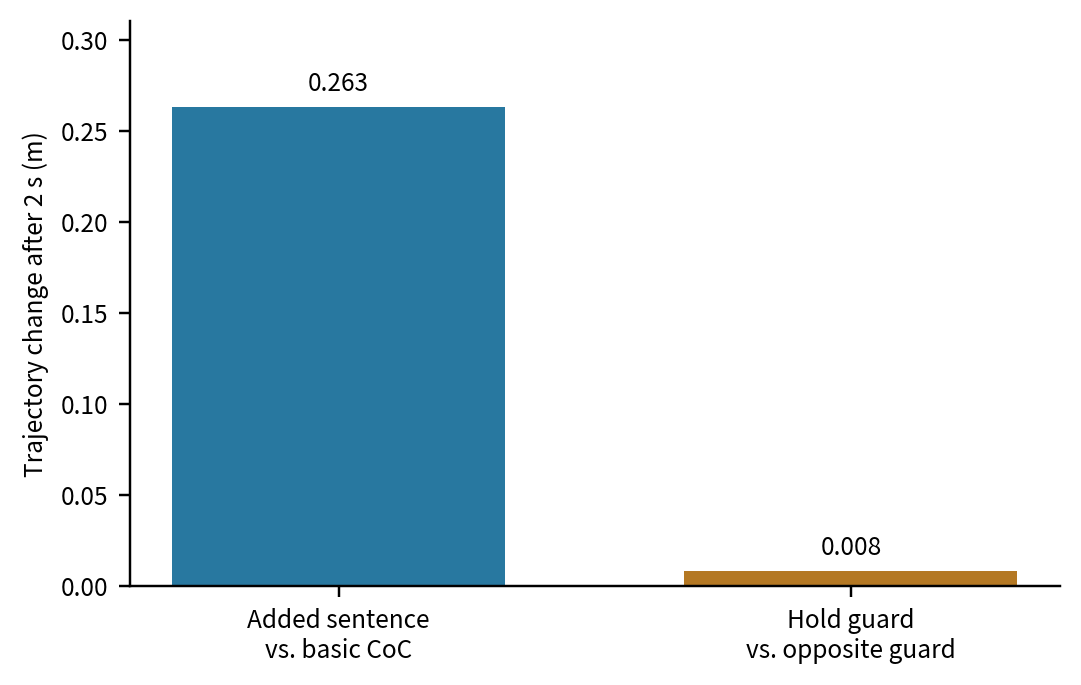
\includegraphics[width=0.94\columnwidth]{../latex-kiee-review-2022/figures/fig04_r1_diagnostic.png}
\bifigcaption{Alpamayo-R1 사전 진단. 첫 막대 0.263 m는 문장을 추가했을 때 기본 CoC와 달라진 정도이므로 `추가 문장에 대한 반응'을 나타낸다. 두 번째 막대 0.008 m는 대기 가드와 반대 가드의 차이이므로 `반대 의미의 구별'을 나타낸다. 두 번째 값이 매우 작아 이 한 장면만으로 의미에 맞는 가드 준수를 확인할 수 없다.}{Alpamayo-R1 pre-training diagnostic: sensitivity to added text is much larger than the trajectory contrast between opposite guard meanings.}
\label{fig:r1-diagnostic}
\end{figure}

\subsection{최소 가드-행동 학습과 초기 과제의 한계}

\paragraph{확인 목적.}
두 번째 실험은 작은 VLM이 "이 가드에서는 정지하고, 저 가드에서는 진행한다"는 대응을 학습할 수 있는지 확인한다. 동시에 정지와 진행만 구분하는 쉬운 문제가 가드의 효과를 실제보다 크게 보이게 할 수 있는지도 확인한다.

\paragraph{비교 방법.}
후보는 정지(STOP)와 진행(PROCEED) 두 가지로 만들었다. 첫 조건에서는 가드와 정답 행동을 올바르게 연결했다. 비교 조건에서는 같은 가드 문장을 사용하되 정답 행동과의 연결을 일부러 섞었다. 이 비교를 통해 모델이 단순히 문장을 받은 효과와 가드의 올바른 의미를 배운 효과를 구분한다. 평가는 학습에 사용하지 않은 장면과, 같은 뜻을 다른 문장으로 표현한 경우로 나누었다. 쉬운 과제에서는 학습량의 차이가 결과에 영향을 주지 않도록 기존 CoC와 CoC+Guard의 학습 횟수도 같게 맞추었다.

\paragraph{결과.}
표준 평가에서 올바른 제약--정답 대응을 학습한 조건의 후보 정확도는 0.990, 계약 쌍 정확도는 0.958이었다. 반면 제약--정답 대응을 교란한 통제군은 각각 0.719와 0.000이었다. 이는 올바른 제약--행동 관계를 학습하면 학습에 쓰지 않은 장면에서도 두 계약을 구별할 수 있음을 보여준다. 그러나 동일 의미 문장 변형 평가에서는 두 조건의 후보 정확도가 0.740과 0.745였고, 계약 쌍 정확도는 모두 0이었다. 즉, 표준 문장과 비슷한 입력에는 대응했지만 같은 뜻의 새로운 표현으로 일반화하지는 못했다.

또한 학습 자료가 충분한 쉬운 과제에서는 기존 CoC만 사용해도 후보 정확도 0.974와 계약 쌍 정확도 0.896에 도달했고, CoC+Guard는 1.000과 1.000이었다. 학습 횟수를 같게 맞춘 사후 비교에서는 두 조건 모두 두 지표가 1.000이었다.

\paragraph{의미.}
두 가지를 알 수 있다. 첫째, 작은 VLM은 가드와 행동의 관계를 학습할 수 있다. 둘째, 쉬운 정지/진행 문제에서는 가드가 없어도 장면만 보고 정답을 외울 수 있다. 이 경우 CoC+Guard의 높은 정확도가 정말 가드를 읽은 결과인지 분명하지 않다. 따라서 정적 실험은 모든 후보가 같은 CoC 목표를 달성하게 만들고, 시간 및 다중 주행 실험은 목표를 완료하는 경쟁 후보에 계속 정지하는 교착 후보를 더하여 가드 준수와 진행성을 함께 측정한다.

\begin{table*}[!t]
\color{reviewerone}
\centering
\bitablecaption{실험 전체의 읽기 안내. 각 행은 연구 질문과 평가 설정, 핵심 비교, 주요 지표 및 증거의 범위를 요약한다. 서로 다른 모델ㆍ과제의 행 사이 수치를 직접 성능 순위로 비교하지 않는다.}{Reading guide summarizing the question and setting, primary comparison, key endpoint, and evidential role of each experiment. Results are interpreted within, not across, rows.}
\label{tab:suite}
\scriptsize
\begin{tabularx}{\textwidth}{L{0.13\textwidth}L{0.22\textwidth}L{0.19\textwidth}L{0.18\textwidth}Y}
\toprule
Experiment & Question and evaluation setting & Primary comparison & Key endpoint & Evidential role \\
\midrule
R1 diagnostic & Does an untrained VLM distinguish opposite guards in one scene? & Basic CoC, hold guard, opposite guard & Trajectory change after 2 s & Text-sensitivity diagnostic; not a compliance test \\
Minimal learning & Can the model learn a correct guard--action mapping on held-out scenes and paraphrases? & Correct versus shuffled mapping & Candidate and paired accuracy & Initial learnability and easy-task limitation \\
Static candidates & Which equal-objective trajectory is admissible under a changed static bound? Standard/paraphrase/unseen-value tests & Basic CoC and four constraint representations & Violation, excess conservatism, paired accuracy & Static constraint-conditioned selection \\
Temporal condition & Does a changed hold duration switch the answer? Standard/paraphrase/unseen-time tests & Short- versus long-hold contracts & Violation, compliant completion, paired accuracy & Temporal release and numeric generalization \\
Stopping/lane change & Does the effect repeat across maneuvers? Standard and combined-shift hard cases & Proposed versus basic and shuffled conditions & Violation, compliant completion, paired accuracy & Multi-constraint and unit/expression robustness \\
Closed-loop auxiliary & Must a released contract be revoked when risk returns? Release-reversal episodes & State, CoC, monotone/dynamic contract, shield & Violation, collision, intervention cost & Reversible state update and runtime checking in a separate small network \\
\bottomrule
\end{tabularx}
\end{table*}

\subsection{동일 목표를 달성하는 정적 궤적 후보}

\paragraph{확인 목적.}
이 실험에서는 모든 후보가 "교차로를 통과한다"는 같은 목표를 달성한다. 따라서 모델은 목표 달성 여부만으로 정답을 고를 수 없다. 현재 가드가 어느 후보를 허용하는지 읽어야 한다.

\paragraph{비교 방법.}
두 후보 모두 교차로를 통과하지만 최대 속도, 장애물과의 최소거리, 진입 시점과 진행 속도가 다르다. 같은 장면에서 완화 계약은 더 빠른 후보를 허용하지만, 엄격 계약은 그 후보를 금지하고 더 신중한 후보를 허용한다. 표~\ref{tab:representations}의 기본 CoC, 제약 통합 CoC, 별도 자연어 제약, 제약--정답 대응 교란 및 논리식 제약을 비교하였다. 두 계약의 정답을 모두 맞혀야 하는 계약 쌍 정확도를 핵심 지표로 사용하였다.

이 정적 결과는 난수 초기값(seed) 42를 사용한 단일 학습 반복이다. 학습 자료는 96개 장면에서 만든 576개 예이고, 분리 평가는 24개 장면에 세 종류의 가드를 각각 쌍으로 적용한 144개 예다. 따라서 표~\ref{tab:static}의 작은 차이를 데이터 생성이나 학습 난수에 대해 안정적인 차이로 해석하지 않는다.

\begin{table*}[!t]
\centering
\bitablecaption{같은 행동 목표를 달성하는 정적 후보의 표준 평가. 후보 정확도와 계약 쌍 정확도는 높을수록 좋고, 가드 위반률과 과도한 보수 선택률은 낮을수록 좋다. 모든 조건의 목표 완료율이 1.000이므로 위반 감소가 목표 포기의 결과는 아니다. 모든 비율은 평가 예 144개를 분모로 한다.}{Standard evaluation of static candidates sharing the same behavioral goal. Accuracy and paired accuracy are higher-is-better; violation and excess conservatism are lower-is-better.}
\label{tab:static}
\footnotesize
\begin{tabularx}{\textwidth}{L{0.22\textwidth}ZZZZZ}
\toprule
Condition & Candidate accuracy & Guard violation rate $\downarrow$ & Excess-conservatism rate $\downarrow$ & Paired-contract accuracy $\uparrow$ & Goal completion rate \\
\midrule
Basic CoC (no constraint) & 0.500 & 0.250 & 0.250 & 0.000 & 1.000 \\
Constraint-integrated CoC (proposed) & \textbf{1.000} & \textbf{0.000} & \textbf{0.000} & \textbf{1.000} & 1.000 \\
Separate natural-language constraint & 0.993 & 0.007 & 0.000 & 0.986 & 1.000 \\
Shuffled constraint--target mapping & 0.465 & 0.188 & 0.347 & 0.153 & 1.000 \\
Logical-form constraint & \textbf{1.000} & \textbf{0.000} & \textbf{0.000} & \textbf{1.000} & 1.000 \\
\bottomrule
\end{tabularx}
\end{table*}

\paragraph{결과.}
표~\ref{tab:static}은 각 행이 무엇을 의미하는지 두 단계로 읽어야 한다. 먼저 마지막 열이 모두 1.000이므로 어느 조건도 교차로 통과 목표를 포기하지 않았다. 그다음 위반률과 계약 쌍 정확도를 보면, 제약 정보가 없는 기본 CoC는 선택의 0.250에서 가드를 위반했고 완화ㆍ엄격 계약을 모두 맞힌 장면은 없어 계약 쌍 정확도가 0.000이었다. 엄격 계약 72개만 분모로 한 원 저장 위반률은 0.500이지만, 다른 표와 정의를 맞추기 위해 여기서는 전체 144개 예 기준인 0.250을 사용하였다. 제약--정답 대응을 교란한 통제군의 계약 쌍 정확도도 0.153에 머물렀다.

반면 제약 통합 CoC와 논리식 제약은 위반률 0.000, 과도한 보수 선택률 0.000, 계약 쌍 정확도 1.000을 기록하였다. 별도 자연어 제약도 전체 예 기준 위반률 0.007과 계약 쌍 정확도 0.986을 기록하였다. 입력 형식이 같은 별도 자연어 제약과 제약--정답 대응 교란의 계약 쌍 정확도 차이 0.833은 제약 문장을 추가하는 것만으로는 부족하고, 올바른 제약--정답 대응을 학습해야 함을 보여준다.

동일 의미 문장 변형 평가의 후보/계약 쌍 정확도는 제약 통합 CoC 0.875/0.750, 별도 자연어 제약 0.924/0.847, 논리식 제약 1.000/1.000이었다. 미관측 수치 평가에서는 각각 1.000/1.000, 0.951/0.903, 0.924/0.847이었다. 여기서 슬래시 앞은 개별 문제의 후보 정확도, 뒤는 같은 장면의 두 계약을 모두 맞힌 계약 쌍 정확도다.

\paragraph{의미.}
제약 통합 CoC는 항상 정지하는 방법으로 위반을 피한 것이 아니다. 모든 후보가 목표를 완료했고, 그중 현재 계약이 허용하는 가장 진행도가 높은 후보를 골랐다. 따라서 이 결과는 모델이 실행 가드를 정적 후보 선택에 사용했음을 보여준다. 다만 정적 과제에서 논리식 제약이 높은 성능을 보였다는 이유만으로 논리 표현이 언제나 더 좋다고 결론 내릴 수는 없다. 다음 시간 과제에서는 다른 결과가 나타난다.

\subsection{정지-대기-해제-출발 시간 조건}

\paragraph{확인 목적.}
앞 실험은 속도나 거리처럼 한 시점의 기준을 다루었다. 이번 실험은 "얼마나 오래 기다려야 하며 언제 출발해도 되는가"라는 시간 조건도 모델이 배울 수 있는지 확인한다.

\paragraph{비교 방법.}
장면과 네 후보는 그대로 두고, 상충 구역이 비어 있는 것을 확인한 뒤 기다려야 하는 시간만 바꾸었다. 완화 계약은 짧게 기다린 뒤 출발하는 후보를 허용하고, 엄격 계약은 더 오래 기다린 후보만 허용한다. 후보는 조기 진입, 짧은 대기 후 진입, 긴 대기 후 진입과 계속 정지로 구성하였다. 각 난수 초기값에서 192개 장면으로 만든 384개 예를 학습하고, 48개 장면으로 만든 96개 계약 예를 평가하였다. 난수 초기값 42, 17, 123은 모델 초기화와 학습 순서뿐 아니라 합성 장면의 값과 후보 문자 배치도 함께 바꾼다. 따라서 세 반복은 전체 절차의 반복성을 보지만, 데이터를 고정한 채 최적화 분산만 분리하지는 않는다. 네 시점을 이어 붙인 연속 장면 영상에는 시각적 상태와 시간이 글자로 표시되고 후보 설명에는 후보 진입 시각이 적혀 있다. 저장한 어댑터를 재학습하지 않고 원본 영상, 정보가 없는 단색 영상, 실제와 다른 `상충 구역이 비기 시작한 시각'을 표시한 충돌 영상으로 각각 다시 평가하여 영상 정보의 기여를 분리하였다.

\begin{table*}[!t]
\centering
\bitablecaption{정지--대기--해제--출발 시간 과제의 표준 평가. 값은 세 난수 초기값 결과의 평균$\pm$모집단 표준편차다. 후보 정확도ㆍ계약 쌍 정확도와 가드 준수 목표 완료율은 높을수록 좋고, 가드 위반률과 교착률은 낮을수록 좋다.}{Standard temporal evaluation for stop--hold--release--go, reported as three-seed mean $\pm$ population standard deviation.}
\label{tab:temporal}
\footnotesize
\begin{tabularx}{\textwidth}{L{0.22\textwidth}ZZZZZ}
\toprule
Condition & Candidate accuracy & Guard violation rate $\downarrow$ & Deadlock rate $\downarrow$ & Guard-compliant goal completion rate $\uparrow$ & Paired-contract accuracy $\uparrow$ \\
\midrule
Basic CoC (no constraint) & $0.500\pm0.000$ & $0.319\pm0.052$ & $0.000\pm0.000$ & $0.681\pm0.052$ & $0.000\pm0.000$ \\
Constraint-integrated CoC (proposed) & $\mathbf{1.000\pm0.000}$ & $\mathbf{0.000\pm0.000}$ & $0.000\pm0.000$ & $\mathbf{1.000\pm0.000}$ & $\mathbf{1.000\pm0.000}$ \\
Separate natural-language constraint & $0.698\pm0.094$ & $0.191\pm0.136$ & $0.000\pm0.000$ & $0.809\pm0.136$ & $0.396\pm0.187$ \\
Shuffled constraint--target mapping & $0.510\pm0.015$ & $0.333\pm0.023$ & $0.000\pm0.000$ & $0.667\pm0.023$ & $0.021\pm0.029$ \\
Logical-form constraint & $0.538\pm0.027$ & $0.274\pm0.108$ & $0.000\pm0.000$ & $0.726\pm0.108$ & $0.076\pm0.055$ \\
\bottomrule
\end{tabularx}
\end{table*}

\paragraph{결과.}
표~\ref{tab:temporal}은 학습과 같은 문장 틀ㆍ시간값 범위를 사용한 표준 평가다. 제약 통합 CoC는 세 번의 반복 모두 가드 위반률 0.000, 가드 준수 목표 완료율 1.000, 계약 쌍 정확도 1.000을 기록하였다. 같은 연속 장면 영상에서 짧은 대기를 요구하면 짧은 대기 후보를, 긴 대기를 요구하면 긴 대기 후보를 골라 두 계약을 모두 맞힌 것이다. 반면 제약 정보가 없는 기본 CoC는 두 계약에 같은 입력을 받으므로 계약 쌍 정확도가 0.000이고 가드 위반률은 $0.319\pm0.052$였다. 별도 자연어 제약은 평균적으로 기본 CoC와 대응 교란 통제군보다 나았지만 난수 초기값에 따라 차이가 컸다. 대응 교란 통제군과 논리식 제약은 두 대기시간의 차이를 안정적으로 배우지 못했다.

\revone{위치만 바꾼 대비에서 제약 통합 CoC와 별도 자연어 제약의 후보 정확도는 각각 1.000과 0.698, 계약 쌍 정확도는 1.000과 0.396이며 가드 위반률은 0.000과 0.191이었다. 반면 같은 별도 필드 형식에서 올바른 대응을 학습한 조건과 대응 교란 조건의 계약 쌍 정확도는 0.396과 0.021이었다. 따라서 전자는 현재 모델에서 목표와 가드를 한 문맥에 배치한 위치ㆍ구획 효과를, 후자는 위치를 고정했을 때 올바른 가드--행동 대응의 효과를 보여준다. 정적 과제에서는 통합/별도 조건의 계약 쌍 정확도가 1.000/0.986으로 위치 효과가 작았으므로, 통합 위치의 이점은 모든 과제에 동일하게 일반화되지 않는다.}

그러나 그림~\ref{fig:temporal-pair}(a)처럼 제약 통합 CoC의 성능은 입력 변화에 따라 낮아졌다. 제약의 뜻과 수치는 같고 말투만 바꾼 \textbf{동일 의미 문장 변형 평가}에서는 후보 정확도 0.858, 가드 위반률 0.115, 가드 준수 목표 완료율 0.885, 계약 쌍 정확도 0.715였다. 문장 틀은 유지하고 학습에 없던 대기시간을 사용한 \textbf{미관측 시간값 평가}에서는 각각 0.635, 0.351, 0.649, 0.306이었다. 즉 문장 표현만 달라져도 성능이 일부 낮아졌고, 새로운 시간값에서는 더 크게 낮아졌다. 표준 평가의 완벽한 결과가 일반적인 시간 비교 규칙의 학습을 의미하지는 않는다.

저장한 세 난수 초기값의 제약 통합 CoC 어댑터를 다시 실행한 원본 영상 결과는 표~\ref{tab:temporal}과 모든 지표에서 정확히 일치하였다. 표~\ref{tab:image-ablation}의 각 셀은 `후보 정확도/계약 쌍 정확도' 순서다. 표준 시간 과제는 원본 1.000/1.000에서 단색 영상 0.670/0.403, 상충 구역이 비기 시작한 시각이 실제와 다른 충돌 영상 0.608/0.340으로 낮아졌다. 단색 영상과 시간 충돌 영상의 가드 위반률도 각각 0.288과 0.208이었다. 따라서 표준 과제의 완벽한 결과는 문장만 읽은 결과가 아니며 연속 장면 영상에 표시된 시간 정보에 의존한다. 반면 미관측 시간값 평가에서는 원본 후보 정확도부터 0.635에 그쳤고 영상 교란이 이를 일관되게 더 낮추지 않았다. 시간 충돌 영상은 문제의 관측 전제 자체를 바꾸므로 그 조건에서 우연히 낮아진 위반률이나 높아진 목표 완료율을 성능 향상으로 해석하지 않는다. 이는 새로운 시간값에서 시각 시간과 수치 관계를 안정적으로 결합하지 못했다는 추가 증거다.

\paragraph{의미.}
제약 통합 CoC는 표준 분포의 같은 장면에서도 제약이 요구하는 대기시간에 따라 출발 후보를 바꾸었다. 그러나 미관측 시간값 결과는 이 대응이 일반적인 시간 비교 규칙으로 충분히 일반화되지 않았음을 보여주므로 RQ4에는 부정적인 답을 준다. 기본 CoC는 두 계약에 동일한 입력을 받으므로 결정적 모델이 두 정답을 모두 구별할 수 없는 정보 부재 기준선이다. 따라서 기본 CoC의 후보 정확도 0.500과 계약 쌍 정확도 0.000을 제안법의 안전성 우월성으로 해석하지 않는다. 시간 과제에서 입력 형식이 같은 별도 자연어 제약과 제약--정답 대응 교란의 계약 쌍 정확도는 각각 0.396과 0.021이었다. 이 차이가 올바른 제약--정답 대응 학습의 더 직접적인 증거다. 반면 제약 통합 CoC와 대응 교란 조건의 차이에는 입력 위치의 효과도 포함된다. 논리식 제약의 낮은 결과도 논리식 자체가 자연어보다 나쁘다는 뜻은 아니다. 두 표현을 공정하게 비교하려면 논리 문법을 별도로 학습시킨 뒤 다시 평가해야 한다.

\subsection{정지ㆍ차선 변경과 복합 표현 변화}

\paragraph{확인 목적.}
앞 실험의 성공이 대기시간 문제에만 나타난 결과일 수 있다. 이를 확인하기 위해 정지와 차선 변경으로 행동을 넓혔다. 또한 같은 가드를 다른 문장이나 처음 보는 수치로 표현해도 모델이 조건을 지키는지 확인하였다.

\paragraph{비교 방법.}
정지 과제에서는 정지선 위치, 최대 감속도와 최대 가가속도를 가드로 사용하였다. 차선 변경 과제에서는 최소 차량 간격과 중단 후 재시도 조건을 사용하였다. 192개 장면마다 완화 계약과 엄격 계약을 하나씩 적용하여 384개 학습 예를 만들었다. 표준 평가, 동일 의미 문장 변형 평가와 미관측 수치 평가는 각각 48개 장면, 즉 96개 계약 문제로 구성하였다. 별도의 \textbf{복합 표현 변화 평가}에는 (1) 측정값이 기준값과 정확히 같은 경계 등호, (2) 부정ㆍ금지 문장, (3) 조건절 순서 변경, (4) 같은 값을 m 대신 cm로 적는 단위 변환을 함께 넣었다. 따라서 이 평가는 네 요인 중 하나의 원인을 분리하는 요인별 실험이 아니라, 여러 표현 변화가 섞인 강건성 시험이다. 저장 어댑터는 원본, 단색 및 반대 행동 종류의 영상에서도 다시 평가하였다.

\revone{표준 평가의 반복적인 1.000이 난이도 부족을 가릴 수 있으므로, 위 복합 표현 변화 평가를 \textbf{hard-case 평가}로 명시하여 행동별로도 재집계하였다. 정지 hard-case는 정지선, 감속도 및 가가속도 세 제약을 동시에 적용하고, 완화 계약의 두 수치 상한을 빠른 후보의 측정값과 정확히 같게 두어 판정 여유가 0인 경계 등호를 포함한다. 차선 변경 hard-case도 완화 계약의 최소 간격을 빠른 후보의 측정값과 같게 두고, 간격 미달 시 중단ㆍ재시도하는 조건을 함께 적용한다. 각 난수 초기값의 48개 장면은 정지와 차선 변경을 24개씩 포함하며, 장면마다 완화ㆍ엄격 계약을 적용한 총 96개 문제다.}

\begin{table*}[!t]
\centering
\bitablecaption{정지ㆍ차선 변경 과제의 표준 평가와 복합 표현 변화 평가. 값은 세 난수 초기값 결과의 평균$\pm$표본 표준편차다. `복합 표현 변화'에는 경계 등호, 부정ㆍ금지, 절 순서 변경 및 m--cm 단위 변환이 함께 포함된다. 단위 정규화 행은 저장 어댑터의 재평가 결과다.}{Standard and combined-expression-shift evaluations for stopping and lane change, including re-evaluation of saved adapters after deterministic unit normalization; values are three-seed mean $\pm$ sample standard deviation.}
\label{tab:maneuver}
\footnotesize
\begin{tabularx}{\textwidth}{L{0.15\textwidth}L{0.22\textwidth}ZZZZ}
\toprule
Evaluation & Condition & Candidate accuracy & Guard violation rate $\downarrow$ & Guard-compliant goal completion rate $\uparrow$ & Paired-contract accuracy $\uparrow$ \\
\midrule
Standard evaluation & Basic CoC (no constraint) & $0.500\pm0.000$ & $0.292\pm0.072$ & $0.708\pm0.072$ & $0.000\pm0.000$ \\
 & Constraint-integrated CoC (proposed) & $\mathbf{1.000\pm0.000}$ & $\mathbf{0.000\pm0.000}$ & $\mathbf{1.000\pm0.000}$ & $\mathbf{1.000\pm0.000}$ \\
 & Shuffled constraint--target mapping & $0.503\pm0.006$ & $0.267\pm0.039$ & $0.733\pm0.039$ & $0.028\pm0.032$ \\
\midrule
Combined expression-shift evaluation & Basic CoC (no constraint) & $0.500\pm0.000$ & $0.302\pm0.065$ & $0.698\pm0.065$ & $0.000\pm0.000$ \\
 & Constraint-integrated CoC (proposed) & $\mathbf{0.948\pm0.063}$ & $\mathbf{0.010\pm0.010}$ & $\mathbf{0.990\pm0.010}$ & $\mathbf{0.896\pm0.127}$ \\
 & \revone{Proposed + unit normalization} & \revone{$\mathbf{0.958\pm0.072}$} & \revone{$\mathbf{0.000\pm0.000}$} & \revone{$\mathbf{1.000\pm0.000}$} & \revone{$\mathbf{0.917\pm0.144}$} \\
 & Shuffled constraint--target mapping & $0.535\pm0.079$ & $0.260\pm0.018$ & $0.740\pm0.018$ & $0.090\pm0.139$ \\
\midrule
\revone{Hard-case by maneuver} & \revone{Proposed: stopping} & \revone{$0.979\pm0.021$} & \revone{$0.021\pm0.021$} & \revone{$0.979\pm0.021$} & \revone{$0.958\pm0.042$} \\
 & \revone{Proposed: lane change} & \revone{$0.917\pm0.144$} & \revone{$0.000\pm0.000$} & \revone{$1.000\pm0.000$} & \revone{$0.833\pm0.289$} \\
\bottomrule
\end{tabularx}
\end{table*}

\paragraph{결과.}
표~\ref{tab:maneuver}의 위쪽 세 행은 표준 평가, 아래쪽 세 행은 복합 표현 변화 평가다. 표준 평가에서 제약 통합 CoC는 정지와 차선 변경 모두 가드 위반률 0.000, 가드 준수 목표 완료율 1.000, 계약 쌍 정확도 1.000을 기록하였다. 즉, 두 행동에서 목표를 완료하면서 완화ㆍ엄격 계약에 따라 정답 후보를 정확히 바꾸었다. 기본 CoC보다 평균 위반률은 0.292 낮았다. 난수 초기값을 단위로 다시 뽑아 계산한 95\% 구간은 [0.250, 0.375]였다. 같은 입력 형식을 사용한 제약--정답 대응 교란 통제군보다 계약 쌍 정확도는 0.972 높았고 해당 구간은 [0.938, 1.000]이었다. 따라서 이 차이는 단순한 제약 문장 추가보다 올바른 제약--정답 대응 학습의 효과를 직접 보여준다. 다만 반복이 세 번뿐이고 각 난수 초기값에서 데이터도 함께 바뀌므로 이 구간은 확정적인 통계 결론이 아니라 전체 절차에서 관찰된 범위를 살펴보는 참고값이다.

복합 표현 변화 평가에서 제약 통합 CoC의 가드 위반률은 $0.010\pm0.010$, 계약 쌍 정확도는 $0.896\pm0.127$로 표준 평가보다 낮아졌다. 오답 15개는 모두 같은 거리를 m 대신 cm로 표현한 문장에서 관찰되었다. 난수 초기값 42의 오답 12개는 가드를 위반하지는 않았지만 필요 이상으로 느린 차선 변경 후보를 선택한 경우였다. 나머지 3개는 난수 초기값 17과 123에서 감속도 또는 가가속도 상한을 넘은 정지 후보를 선택한 경우였다. 부정 표현, 조건절 순서 변경과 m 단위 경계값만 포함한 예에서는 오답이 없었다. 그러나 여러 변화가 한 평가 집합에 함께 있으므로 이 관찰만으로 단위 변환이 유일한 원인이라고 확정할 수는 없다.

\revone{단위 정규화 효과를 분리하기 위해 저장된 세 어댑터와 동일한 288개 hard-case 문제를 다시 사용하고, 72개 cm 문장의 수치와 단위만 동등한 m 표현으로 결정적으로 변환한 뒤 재평가하였다. 장면, 후보, 정답, 나머지 문장 및 모델 가중치는 바꾸지 않았다. cm 부분집합의 정답은 57/72(0.792)에서 60/72(0.833)로 3건 회복되었고 회귀한 정답은 없었다. 이에 따라 전체 후보 정확도는 0.948에서 0.958, 계약 쌍 정확도는 0.896에서 0.917로 높아졌으며, 세 건의 안전하지 않은 정지 선택이 모두 교정되어 가드 위반률은 0.010에서 0.000으로 낮아졌다. 그러나 난수 초기값 42의 과도하게 보수적인 차선 변경 오답 12건은 남았다. 비-cm 입력의 예측은 하나도 변하지 않았다. 따라서 단위 정규화는 수치 안전 오류를 제거하는 실용적인 전처리였지만, 복합 문장에 대한 보수적 선택까지 해결하지는 못했다.}

\revone{행동별 hard-case에서 제약 통합 CoC의 후보/계약 쌍 정확도는 정지 0.979/0.958, 차선 변경 0.917/0.833이었다. 정지의 가드 위반률은 0.021이었고 차선 변경의 가드 위반률은 0이었지만, 차선 변경에서는 가드를 지키면서도 더 느린 후보를 고른 과도한 보수 선택 때문에 계약 쌍 정확도가 더 낮았다. 이 하락은 표준 평가의 1.000을 일반적인 난제 해결 성능으로 해석할 수 없고, 동시 제약ㆍ경계 등호ㆍ표현 변화가 모델 차이를 드러내는 데 필요함을 보여준다.}

다중 주행의 표준 평가와 미관측 수치 평가는 단색 영상과 반대 행동 영상에서도 세 난수 초기값 모두 후보 정확도와 계약 쌍 정확도 1.000을 유지하였다. 복합 표현 변화 평가의 원본/단색/반대 행동 영상은 각각 후보 정확도 0.948/0.906/0.948, 계약 쌍 정확도 0.896/0.813/0.896이었다. 이 과제의 영상은 행동 종류별 고정 도식이고 후보 물리량과 행동 종류가 문장에 직접 적혀 있으므로, 높은 표준ㆍ미관측 수치 결과는 시각적 근거화가 아니라 주로 문장 기반 제약 후보 선택의 증거다.

\begin{table*}[!t]
\centering
\bitablecaption{저장 어댑터의 영상 절제 재평가. 각 셀은 `후보 정확도/계약 쌍 정확도' 순서의 세 난수 초기값 평균이다. 단색 영상은 시각 정보를 제거한다. 충돌 영상은 시간 과제에서 상충 구역이 비기 시작한 시각을 실제와 다르게 표시하고, 다중 주행 과제에서는 문장과 반대되는 행동 도식을 제시한다. 충돌 영상은 입력 전제를 바꾸므로 강건성 향상이 아니라 영상 의존성 진단으로만 읽는다.}{Image-ablation re-evaluation of saved adapters. Each cell reports candidate accuracy/paired-contract accuracy averaged over three seeds.}
\label{tab:image-ablation}
\footnotesize
\begin{tabular}{llccc}
\toprule
Task & Evaluation & Original image & Blank image & Conflicting image \\
\midrule
Temporal & Standard evaluation & 1.000/1.000 & 0.670/0.403 & 0.608/0.340 \\
 & Unseen-time-value evaluation & 0.635/0.306 & 0.691/0.382 & 0.705/0.410 \\
Stopping and lane change & Standard evaluation & 1.000/1.000 & 1.000/1.000 & 1.000/1.000 \\
 & Combined expression-shift evaluation & 0.948/0.896 & 0.906/0.813 & 0.948/0.896 \\
\bottomrule
\end{tabular}
\end{table*}

\paragraph{의미.}
제약을 CoC 안에 함께 제시하는 효과는 대기시간뿐 아니라 정지와 차선 변경에서도 나타났다. 그러나 복합 표현 변화 평가에서는 오류가 남았다. 오답이 cm 표현에 집중되었더라도 여러 변화가 함께 포함된 평가이므로 모든 오류의 원인이 단위 변환이라고 확정할 수는 없다. 후속 실험에서는 단위, 부정 표현, 조건 순서와 경계값을 한 번에 하나씩만 바꾸어 원인을 분리해야 한다.

\begin{figure*}[!t]
\centering
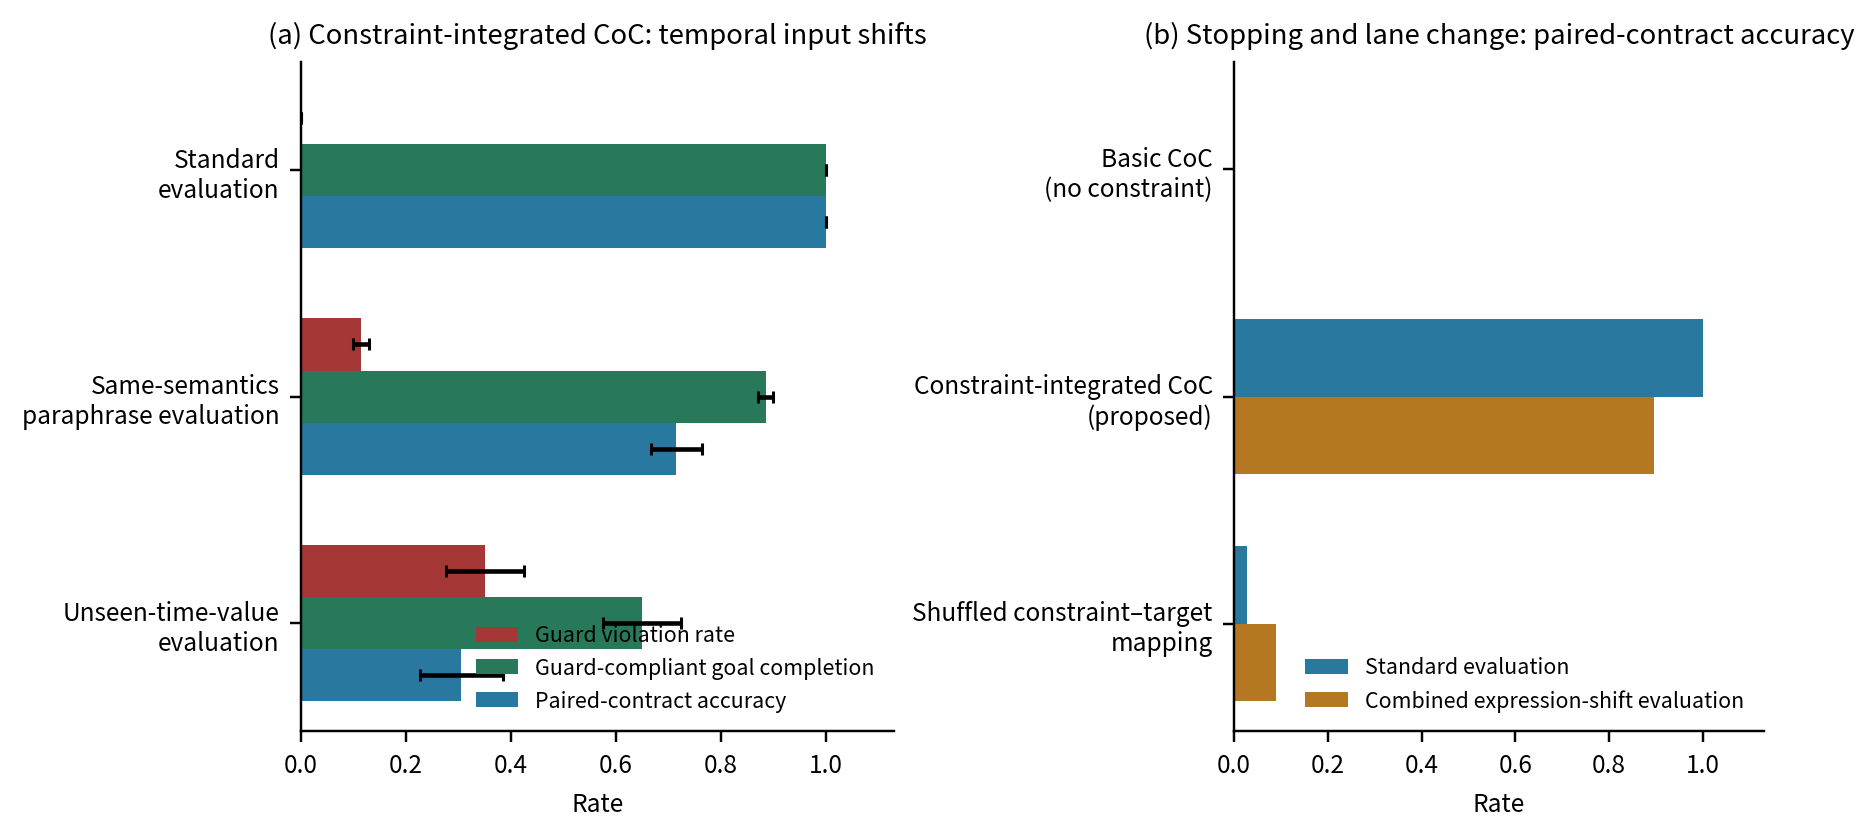
\includegraphics[width=0.98\textwidth]{../latex-kiee-review-2022/figures/fig05_temporal_pair.png}
\bifigcaption{입력 변화에 따른 성능. (a)는 제약 통합 CoC의 시간 과제를 비교한다. 빨간색 가드 위반률은 낮을수록, 초록색 가드 준수 목표 완료율과 파란색 계약 쌍 정확도는 높을수록 좋다. 표준 평가에서는 위반률 0.000, 나머지 두 지표 1.000이지만 동일 의미 문장 변형 평가에서 낮아지고, 미관측 시간값 평가에서 가장 크게 낮아진다. (b)는 정지ㆍ차선 변경 과제의 계약 쌍 정확도다. 파란색은 표준 평가, 주황색은 경계ㆍ부정ㆍ순서ㆍ단위 변화가 함께 든 복합 표현 변화 평가다. 기본 CoC와 대응 교란 통제군은 낮고 제약 통합 CoC만 두 평가에서 높은 값을 유지한다. (a)의 오차 막대는 모집단 표준편차이며 (b)의 표 값은 표본 표준편차를 사용한다.}{Performance under input shifts. Panel (a) shows temporal degradation from standard to paraphrased and unseen-time evaluations; panel (b) compares paired-contract accuracy under standard and combined expression shifts.}
\label{fig:temporal-pair}
\end{figure*}

\subsection{폐루프 보조 실험}

\paragraph{확인 목적.}
앞의 실험은 VLM이 미리 주어진 후보를 한 번 선택하는 문제였다. 마지막 실험은 선택 뒤에도 상황이 계속 바뀌는 경우를 살펴본다. 학습된 계약만 사용할 때와, 실행 중 위험한 명령을 막는 차단 장치를 함께 사용할 때를 비교한다. 이 실험은 작은 신경망과 단순한 운동 모델을 사용한 보조 분석이며, 앞의 VLM 결과나 실제 차량과 직접 비교하지 않는다.

\paragraph{비교 방법.}
두 층 신경망과 1차원 운동학으로 만든 소규모 폐루프 환경을 사용하였다. 폐루프란 모델이 한 번만 답하는 것이 아니라, 매 시점의 상태를 다시 받아 다음 행동을 계속 정하는 환경을 뜻한다. \textbf{상태 전용(State only)}은 수치 상태만, \textbf{상태+CoC(State + CoC)}는 상태와 행동 목표를 입력한다. \textbf{동적 계약(Dynamic contract)}은 현재 위험에 따라 대기와 출발 허용을 양방향으로 갱신한다. \textbf{단조 단계 계약(Monotone-stage contract)}은 한 번 출발을 허용하면 위험이 다시 생겨도 대기로 돌아가지 않는다. \textbf{계약+차단장치(Contract + shield)}는 동적 계약에 더해 실행 직전 위험한 명령을 막는다. 그림의 \textit{Delayed} 조건은 계약 정보가 실제 상태보다 0.4초 늦게 도착한 경우다.

\revone{해제 후 재위험 episode의 핵심 상태전이는 $\mathrm{HOLD}\rightarrow\mathrm{RELEASED}\rightarrow\mathrm{HOLD}$이다. $t=0$에 출발이 허용되더라도 $t=0.8$에 다른 차량이 다시 나타나면 기존 허용을 취소하고 대기 가드를 재활성화해야 한다. 동적 계약은 현재 위험을 반영하여 이 역전이를 표현하지만, 단조 단계 계약은 $\mathrm{RELEASED}$에 고정되어 현재 허용 범위를 잘못 나타낸다. 따라서 이 비교는 계약에 해제 조건만 두는 것으로 충분한지, 해제 이후에도 센서 상태에 따라 가드를 되살리는 reversible update가 필요한지를 평가한다.}

평가는 두 상황으로 나누었다. 첫째, 학습 자료에 정지, 대기, 출발 등 모든 주행 단계가 충분히 들어 있는 상황이다. 둘째, 출발이 허용된 뒤 다른 차량이 다시 나타나므로 다시 정지해야 하지만 학습에서는 보지 못한 "해제 후 위험 재등장" 상황이다. 앞으로 1.2초의 모든 상황을 미리 아는 조건도 넣었지만, 이는 실제 방법이 아니라 도달 가능한 가장 좋은 결과를 보기 위한 참고값이다.

\revone{차단장치의 비용은 episode당 평균 개입 횟수뿐 아니라 동일한 300개 episode bank에서 차단장치가 없는 계약 조건 대비 평균 진행거리와 평균 절대 가가속도의 변화로 측정하였다. 진행거리 감소는 효율 손실의 대리 지표이고 가가속도 증가는 승차감 비용의 대리 지표다. 이 평가는 개별 개입이 반드시 필요했는지를 판정하는 독립 oracle을 포함하지 않으므로, 개입 횟수를 개별 불필요 개입률로 해석하지 않는다.}

\begin{figure*}[!t]
\centering
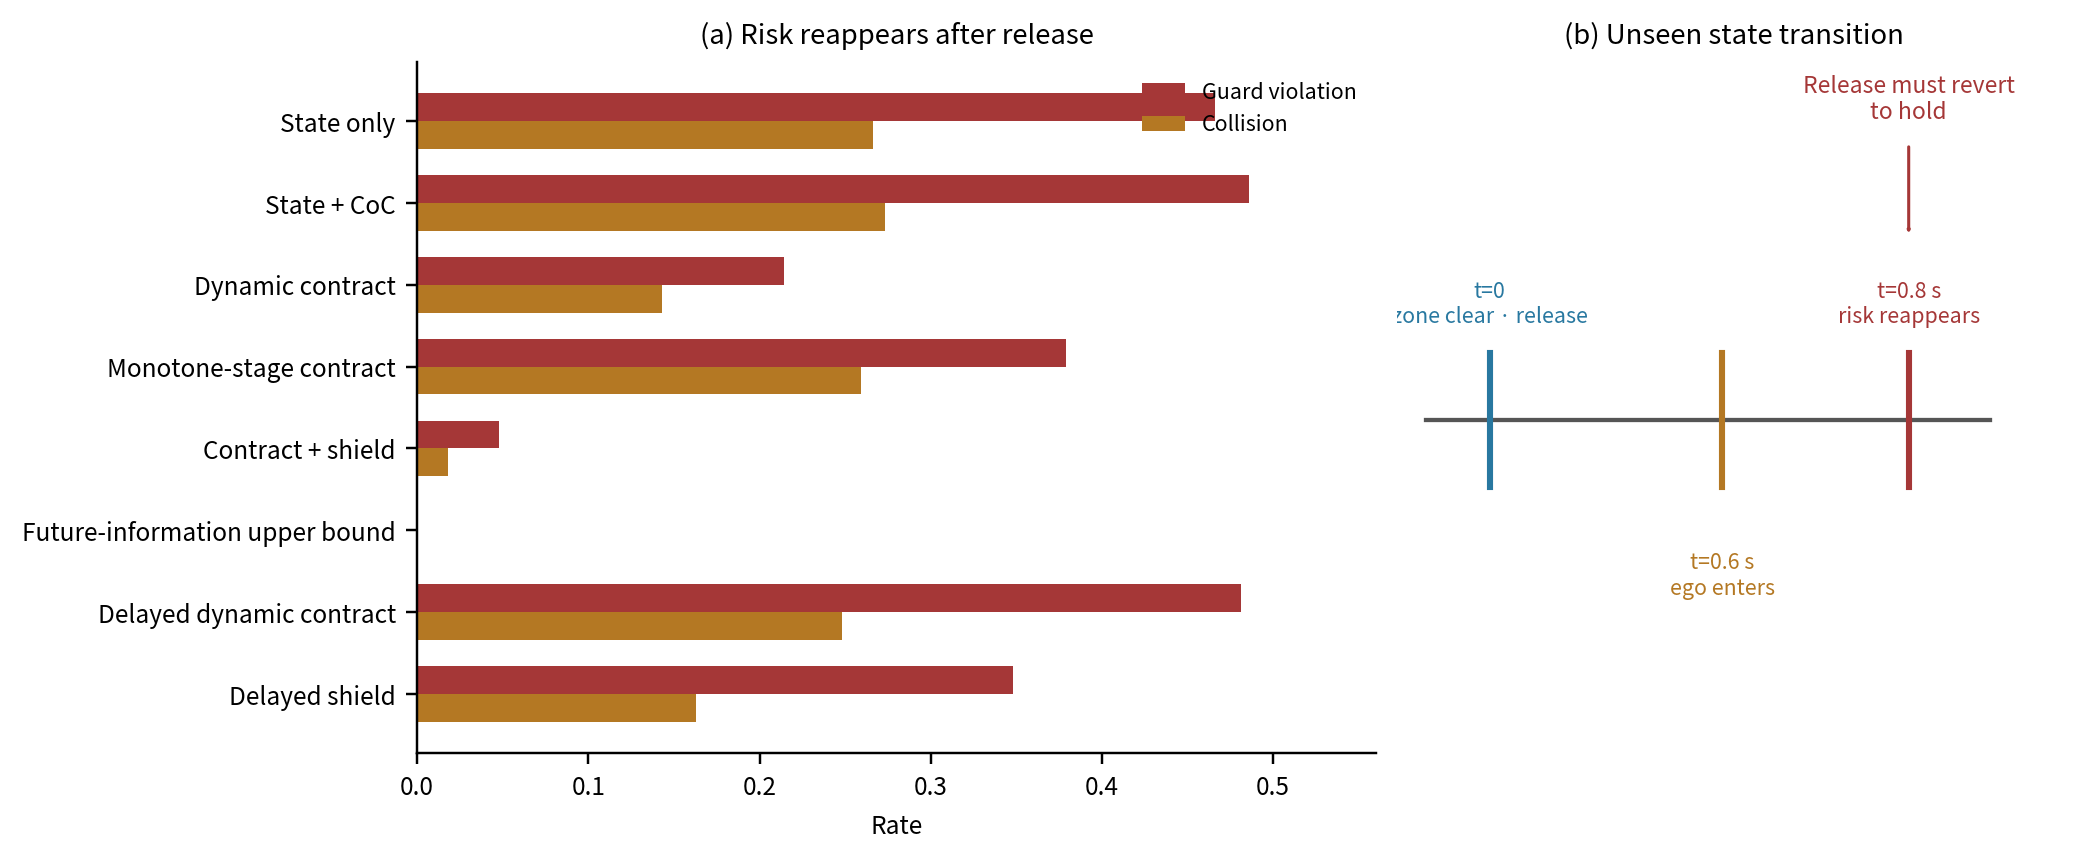
\includegraphics[width=0.98\textwidth]{../latex-kiee-review-2022/figures/fig06_release_reversal.png}
\bifigcaption{폐루프 보조 실험. (a)의 빨간 막대는 가드 위반률, 주황 막대는 충돌률이며 둘 다 낮을수록 좋다. 출발 허용 뒤 위험이 다시 나타날 때 상태 전용과 상태+CoC는 약 0.47--0.49의 위반률을 보이고, 최신 동적 계약은 0.214, 계약+차단장치는 0.048로 낮춘다. 계약 정보가 0.4초 늦으면 다시 악화된다. (b)는 $t=0$ 출발 허용, $t=0.6$ ego 진입, $t=0.8$ 위험 재등장 순서와 다시 대기로 돌아가야 하는 이유를 보여준다. 미래정보 상한은 앞 상황을 완벽히 안다는 비현실적 참고값이다.}{Auxiliary closed-loop experiment showing lower-is-better guard-violation and collision rates when risk reappears after release, together with the event timeline.}
\label{fig:release-reversal}
\end{figure*}

\paragraph{결과.}
먼저 모든 주행 단계를 학습한 상황을 보았다. 정지 후 대기로 넘어가는 예 1,404개를 학습 자료에 추가하자 상태 전용, 상태+CoC, 동적 계약과 단조 단계 계약 모두 300회 평가에서 정지 구간에 너무 일찍 들어가지 않았다. 학습 분포 밖 상황의 가드 위반률도 상태 전용 2.6\%, 상태+CoC 1.4\%, 동적 계약, 단조 단계 계약과 계약+차단장치는 모두 0\%였다. 이 경우 차단장치는 위반률을 더 낮추지 못했지만 주행할 때마다 평균 2.539회 개입했다. 이미 학습으로 해결된 상황에서는 차단장치가 불필요하게 작동할 수 있음을 뜻한다.

그러나 그림~\ref{fig:release-reversal}의 해제 후 재위험 상황에서는 결과가 달랐다. 가드 위반률은 상태 전용 46.6\%, 상태+CoC 48.6\%, 동적 계약 21.4\%, 단조 단계 계약 37.9\%, 계약+차단장치 4.8\%였다. 동적 계약은 현재 위험 상태를 알려 주어 위반을 줄였고, 차단장치는 위험한 행동을 실행 직전에 막아 위반을 더 줄였다. 충돌률도 같은 순서로 26.6\%, 27.3\%, 14.3\%, 25.9\%, 1.8\%였다.

\revone{같은 해제 후 재위험 bank에서 동적 계약은 단조 단계 계약보다 가드 위반률을 16.5\%p(37.9\%에서 21.4\%), 충돌률을 11.6\%p(25.9\%에서 14.3\%) 낮췄다. 두 조건은 모두 목표 완료율 100\%였으므로 이 차이는 영구 정지로 얻은 결과가 아니다. 단조 상태가 과거의 출발 허용을 유지하는 동안 동적 상태는 재등장한 위험에 맞추어 대기 가드를 다시 제공한다는 차이가 성능 격차와 일치한다. 다만 동적 계약도 위반을 없애지는 못했으므로 reversible update는 필요한 정보 갱신이지 그 자체로 실행 안전 보장은 아니다.}

모든 조건의 목표 완료율은 100\%였으므로 낮은 위반률이 단순히 차량을 계속 세운 결과는 아니었다. 앞으로의 상황을 완벽히 아는 비현실적 조건만 위반과 충돌이 모두 0\%였다. 또한 계약 정보가 실제 상황보다 0.4초 늦게 도착하면 동적 계약의 위반률은 48.1\%, 계약+차단장치는 34.8\%로 증가하였다. 올바른 계약도 늦게 전달되면 효과가 크게 줄어든다는 뜻이다.

\begin{table*}[!t]
\color{reviewerone}
\centering
\bitablecaption{차단장치의 안전 이득과 개입 비용. 값은 세 난수 초기값 평균이며, 변화량은 차단장치가 없는 대응 계약 대비 차단장치 조건의 차이다. 모든 조건의 목표 완료율은 1.000이었다.}{Safety benefit and intervention cost of the shield. Deltas compare each shielded condition with its corresponding unshielded contract condition; all completion rates were 1.000.}
\label{tab:shield-cost}
\footnotesize
\begin{tabularx}{\textwidth}{L{0.18\textwidth}L{0.18\textwidth}ZZZZ}
\toprule
Evaluation bank & Comparison & Violation/collision change & Interventions per episode & Progress change (m) & Mean absolute jerk change \\
\midrule
Phase-complete ID & Phase contract $\rightarrow$ shield & $0.000/0.000$ & 1.269 & $-0.076$ & $+0.065$ \\
Phase-complete OOD & Phase contract $\rightarrow$ shield & $0.000/0.000$ & 2.539 & $-0.078$ & $+0.040$ \\
Release-reversal & Dynamic contract $\rightarrow$ shield & $-0.166/-0.125$ & 9.935 & $-0.030$ & $+0.306$ \\
\bottomrule
\end{tabularx}
\end{table*}

\revone{표~\ref{tab:shield-cost}에서 모든 주행 단계를 학습한 phase-complete bank의 ID와 OOD 조건은 차단장치 없이도 위반과 충돌이 0이었다. 차단장치는 추가적인 이진 안전 이득 없이 episode당 각각 1.269회와 2.539회 개입했고, 평균 진행거리를 0.076 m와 0.078 m 줄이며 평균 절대 가가속도를 0.065와 0.040 높였다. 반면 해제 후 재위험 bank에서는 episode당 9.935회의 개입과 함께 동적 계약 대비 위반률을 0.166, 충돌률을 0.125 낮추었고, 진행거리 0.030 m 감소와 평균 절대 가가속도 0.306 증가가 동반되었다. 따라서 차단장치는 미관측 재위험에서 안전 이득을 제공했지만, 이미 이진 안전지표가 포화된 bank에서는 이득 없이 보수적 개입 비용만 발생했다.}

\paragraph{의미.}
이 소규모 폐루프 환경에서는 충분한 성공 시연이 있을 때 문장에 적히지 않은 일부 제약도 행동 예에서 학습되었다. 이때 차단장치를 항상 사용하면 위반률을 더 낮추지 못하면서 개입만 늘어날 수 있었다. 그러나 학습하지 않은 위험이 다시 나타나면 동적 계약만으로는 위반을 모두 막지 못했다. 최신 상태를 사용하는 차단장치를 함께 사용했을 때 위반과 충돌이 가장 크게 줄었고, 그 효과도 계약 정보가 늦으면 감소했다. 이는 별도 미시 환경에서 실행 검사와 정보 최신성의 역할을 보여주는 결과이며, Qwen VLM이나 실제 차량에서 같은 감소율을 기대할 근거는 아니다.

\revone{그러므로 실제 시스템 관점의 비교는 위반ㆍ충돌 감소만으로 끝나지 않고 개입 빈도, 진행 손실 및 승차감 대리 지표를 함께 보고해야 한다. 본 실험은 개입 비용을 정량화했지만 개별 개입의 필요성을 판정하는 독립 oracle은 없으므로 intervention precision은 후속 평가 과제로 남는다.}

\flushbottom
\section{논의와 연구 범위}
\label{sec:discussion}

본 장에서는 5장의 결과가 무엇을 뜻하는지, 그리고 그 결과를 어디까지 해석할 수 있는지 설명한다. 핵심은 기본 CoC를 실행 가드로 보완하는 학습과, 실제 실행 단계에서 궤적을 다시 검사하는 일을 구분하는 것이다.

\subsection{기본 CoC와 실행 가드가 맡는 역할}

기본 CoC는 "보행자에게 양보한 뒤 진행한다"처럼 달성할 행동과 그 이유를 설명한다. 실행 가드는 "정지선을 넘지 않는다" 또는 "상충 구역이 1.5초 동안 비어 있을 때만 출발한다"처럼 그 행동을 언제, 어느 범위에서 허용할지를 정한다. Safety-Constrained CoC는 이 두 정보를 한 문맥에 넣은 \textbf{제약 통합 CoC}이며, 영어로만 작성한 표와 그림 내부에서는 \textit{Constraint-integrated CoC (proposed)}로 표시하였다.

표준 시간 과제에서 기본 CoC(제약 없음)의 가드 위반률은 0.319였지만 제약 통합 CoC는 0.000이었다. 이 결과는 기본 CoC가 위험하다는 뜻이 아니다. 기본 CoC에는 짧게 기다릴지 길게 기다릴지를 구분할 정보가 없었고, 동일 입력에 서로 다른 정답이 연결되므로 후보 정확도 0.500과 계약 쌍 정확도 0.000은 구조적으로 예상된다. 실행 가드를 추가하고 올바른 후보와 함께 학습했을 때 모델이 표준 분포에서 그 차이를 배울 수 있었다는 것이 정확한 해석이다. 따라서 본 논문의 기여는 기존 CoC를 부정하는 것이 아니라, CoC가 말하지 않은 허용 조건을 학습 가능한 형태로 보완하고 그 사용 여부를 쌍대 계약으로 측정하는 데 있다.

\revtwo{이 관점에서 제안 방법의 비교 우위는 더 큰 범용 주행 모델을 만드는 데 있지 않다. 행동 목표와 허용조건을 분리해 사람이 읽을 수 있게 하고, 같은 장면의 가드만 바꾸어 조건 사용 여부를 진단하며, 모델 외부 검증으로 위반ㆍ목표 포기ㆍ과도한 보수성을 구별할 수 있다는 데 있다. 표준 시간 평가에서 위반률 0.000, 가드 준수 목표 완료율 1.000 및 계약 쌍 정확도 1.000이 동시에 나타난 것은 이 세 판정이 서로 모순되지 않았음을 보여준다. 다만 미관측 시간값에서 세 지표가 함께 악화되었으므로 이 장점은 현재 합성 표준 분포에서 확인된 진단적 장점으로 한정한다.}

\subsection{제약 통합 CoC가 높은 결과를 보인 이유}

\revone{표준 시간 과제의 position-only ablation에서 제약 통합 CoC와 별도 자연어 제약은 같은 가드 문장ㆍ학습 예ㆍ학습량을 사용했지만 계약 쌍 정확도가 각각 1.000과 0.396이었다. 이는 현재 시간 과제에서 목표와 가드를 한 문맥에 놓는 위치ㆍ구획 방식이 크게 작용했음을 보여주며, 의미 학습만의 효과로 해석할 수 없다. 한편 위치를 별도 필드로 고정하면 올바른 대응과 대응 교란의 계약 쌍 정확도가 0.396과 0.021이므로, 위치 효과와 별개로 올바른 가드--행동 대응도 필요했다. 다만 통합 위치의 대응 교란 조건이 없는 불완전한 요인 설계이고, 정적 과제의 통합/별도 차이는 1.000/0.986으로 작았다. 따라서 현재 증거는 통합 위치의 보편적 우월성이 아니라 과제 의존적 위치 효과와 의미 대응 효과가 모두 존재함을 지지한다. 제약 통합 CoC도 동일 의미 문장 변형 평가에서 계약 쌍 정확도 0.715, 미관측 시간값 평가에서 0.306으로 낮아졌으므로 표준 분포의 높은 성능을 일반적인 시간 추론 능력으로 볼 수 없다.}

그러나 이 결과만으로 자연어가 논리식보다 본질적으로 우수하다고 결론 내릴 수는 없다. 정적 후보 실험에서는 논리식 제약도 위반률 0.000과 계약 쌍 정확도 1.000을 기록하였다. 표현 방식을 공정하게 비교하려면 논리 문법을 따로 학습시키고, 각 조건에 같은 양의 학습 자료와 학습 횟수를 제공한 뒤 다시 평가해야 한다. 현재 결과가 직접 보여주는 것은 자연어의 보편적 우수성이 아니라, 현재 VLM과 학습 조건에서는 제약 통합 CoC가 가장 안정적이었다는 점이다.

\subsection{수치 조건은 모델 외부 검증기가 다시 확인해야 한다}

다중 주행의 복합 표현 변화 평가에서 관찰된 오답 15개는 모두 같은 거리를 m 대신 cm로 표현한 문장에서 발생하였다. 그러나 경계 등호, 부정ㆍ금지, 절 순서 및 단위 변화가 한 평가에 함께 있으므로 단위 변환만을 유일한 원인으로 분리한 결과는 아니다. 더구나 시간 과제의 미관측 시간값 평가에서도 위반률이 0.351로 증가하였다. 모델이 새로운 수치와 단위를 항상 정확하게 처리한다고 볼 수 없으므로, 실제 적용에서는 모델에 모든 계산을 맡기지 않고 그림~\ref{fig:future-architecture}과 같이 역할을 나누는 것이 적절하다.

먼저 모델은 자연어 Safety-Constrained CoC에서 행동 목표와 실행 가드의 의미를 읽는다. 다음 단계에서는 "최소 간격 600 cm"를 조건 종류, 비교 방향, 값과 단위로 나눈다. 그 뒤 600 cm를 6.0 m처럼 기준 단위로 통일한다. 마지막으로 모델 외부 결정적 검증기 또는 차단장치가 선택한 궤적의 거리, 속도와 시간 조건을 수치로 검사한다.

\revone{저장 어댑터의 재평가는 이 구조의 실용적 이점과 한계를 함께 보여준다. cm 경계만 동등한 m 값으로 바꾸자 세 건의 안전하지 않은 선택이 모두 교정되어 가드 위반률은 0.010에서 0.000으로 낮아졌지만, 후보 정확도와 계약 쌍 정확도의 향상은 각각 0.010과 0.021에 그쳤다. 남은 12건은 모두 안전하지만 과도하게 보수적인 차선 변경 선택이었다. 즉 결정적 단위 정규화는 모델에 생소한 단위 계산을 맡기지 않아 수치 위반을 줄일 수 있지만, 부정 표현ㆍ절 순서ㆍ경계 등호가 결합된 문장의 선택 편향까지 없애지는 않는다.}

이 과정에서는 "미만"과 "이하"처럼 경계값 포함 여부를 구분해야 한다. 또한 가드를 지킬 수 없을 때 정지할지, 다시 기다릴지와 같은 대체 행동도 정해야 한다. 모델은 문장의 목표와 조건을 해석하고, 검증기는 정확한 수치 경계를 확인하도록 역할을 나누는 것이다.

\begin{figure}[t]
\centering
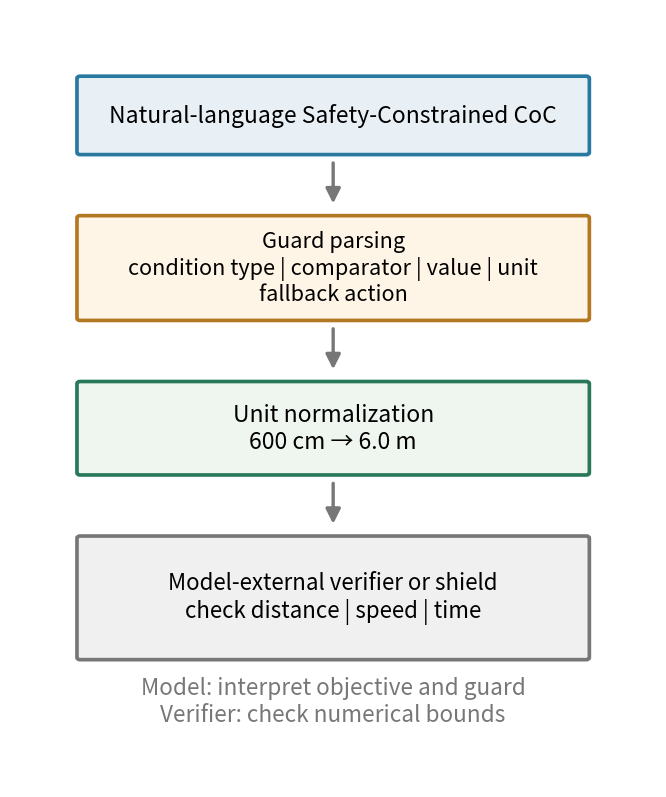
\includegraphics[width=0.94\columnwidth,trim=18 22 18 22,clip]{../latex-kiee-review-2022/figures/fig05_typed_contract.png}
\bifigcaption{자연어 실행 가드를 실제 검사에 연결하는 네 단계. 위에서 아래로 (1) 자연어 제약 통합 CoC를 읽고, (2) 조건 종류ㆍ비교 방향ㆍ값ㆍ단위ㆍ대체 행동으로 나누며, (3) 600 cm를 6.0 m처럼 기준 단위로 통일하고, (4) 모델 외부 검증기 또는 차단장치가 선택한 궤적의 거리ㆍ속도ㆍ시간을 수치 경계와 비교한다. 모델은 목표와 가드를 해석하고 결정적 검증기는 정확한 수치 판정을 담당한다.}{Four-stage path from a natural-language execution guard to typed fields, unit normalization, and deterministic runtime verification.}
\label{fig:future-architecture}
\end{figure}

\subsection{학습된 가드와 실행 차단장치는 역할이 다르다}

가드를 학습하면 모델이 가드를 지키는 후보를 선택할 가능성이 높아진다. 그러나 학습에서 보지 못한 모든 상황에서 준수를 보장하지는 않는다. 폐루프의 해제 후 재위험 상황에서 동적 계약은 가드 위반률을 46.6\%에서 21.4\%로 줄였지만 위반을 없애지는 못했다. 최신 상태를 사용하는 차단장치를 함께 적용했을 때 위반률은 4.8\%까지 낮아졌다. 이는 학습된 계약과 실행 단계 검사가 서로 다른 역할을 맡는다는 것을 보여준다.

차단장치도 모든 문제를 해결하지는 못한다. 계약 정보가 0.4초 늦게 도착했을 때 계약+차단장치의 위반률은 34.8\%로 증가하였다. 계약 자체가 틀리거나 중요한 위험이 빠져 있어도 차단장치는 잘못된 조건을 정확하게 집행할 뿐이다. 따라서 실제 시스템에서는 위험이 다시 나타나면 출발 허용을 취소하고 대기 상태로 돌아갈 수 있어야 한다. 계약이 어느 시점의 상황을 설명하는지도 확인해야 하며, 미래 상황이 불확실하면 더 신중한 대체 행동을 선택해야 한다.

\revone{동적 계약과 단조 단계 계약의 차이는 이 갱신 요구를 직접 드러낸다. 출발 허용은 영구적인 단계 완료가 아니라 현재 관측에 의존하는 임시 허가이므로, 위험이 재등장하면 계약 상태도 $\mathrm{RELEASED}$에서 $\mathrm{HOLD}$로 되돌아가야 한다. 이 역전이를 허용한 동적 계약은 단조 단계 계약보다 위반률을 16.5\%p, 충돌률을 11.6\%p 낮췄다. 반대로 계약 갱신이 0.4초 늦어지면 동적 계약의 위반률이 48.1\%로 악화된 결과는 상태의 가역성뿐 아니라 최신성도 필요함을 보여준다. 이 결과는 별도 소형 폐루프 환경의 메커니즘 증거이며 실제 차량에서 같은 감소폭을 보장하지 않는다.}

\revone{또한 표~\ref{tab:shield-cost}은 차단장치의 가치를 안전 이득과 비용으로 함께 판단해야 함을 보여준다. 해제 후 재위험에서는 위반ㆍ충돌 감소가 있었지만 episode당 9.935회 개입과 가가속도 증가가 동반되었다. 반대로 phase-complete bank에서는 1.269--2.539회 개입하고 진행거리와 가가속도가 소폭 악화되었지만 추가적인 이진 안전 이득은 없었다. 그러므로 차단장치는 상시적인 무비용 보장 장치가 아니라, 학습 정책의 잔여 위험과 개입 비용을 함께 측정하여 적용 범위를 정해야 하는 구성요소다.}

\subsection{주 실험이 실제로 확인한 것}

주 실험은 모델이 연속 궤적을 새로 생성하는 문제가 아니다. 합성 이미지와 수치가 적힌 궤적 후보를 주고 그중 하나를 선택하게 한 실험이다. 따라서 이 실험이 직접 확인한 것은 모델 입력에 포함된 실행 가드가 후보 선택에 조건으로 사용될 수 있는가이다. 입력 형식을 맞춘 비교에서 올바른 대응 학습의 계약 쌍 정확도가 제약--정답 대응 교란보다 높았다는 결과가 이 주장을 가장 직접적으로 뒷받침한다. 정적ㆍ시간 과제에서는 별도 자연어 제약과 대응 교란을, 다중 주행 과제에서는 제약 통합 CoC와 대응 교란을 비교해야 한다. 입력 형식이 다른 조건의 차이를 올바른 대응 관계만의 효과로 해석하지 않는다.

쌍대 계약은 같은 장면에서 가드만 바꾸므로 장면만 보고 같은 답을 반복하는 방법을 막는다. 가드 준수 목표 완료율은 모델이 가드 위반을 피하려고 끝까지 정지하는 방법도 막는다. 이 두 지표를 함께 사용하면 모델이 행동 목표를 끝내면서 가드에 맞는 후보를 골랐는지 확인할 수 있다. 영상 절제에서는 표준 시간 과제의 후보 정확도가 원본 1.000에서 단색 영상 0.670과 `상충 구역이 비기 시작한 시각'이 실제와 다른 충돌 영상 0.608로 낮아져 합성 연속 장면 영상의 시간 정보 사용이 확인되었다. 그러나 다중 주행의 표준ㆍ미관측 수치 평가는 단색 및 반대 행동 영상에서도 1.000을 유지하였다. 즉 영상 의존성은 과제별로 달랐고, 다중 주행의 높은 점수는 문장에 적힌 행동 종류와 후보 수치만으로 설명된다. 시간 과제도 글자가 그려진 합성 연속 장면 영상이므로 실제 센서 장면의 시각적 근거화로 일반화할 수 없다. 후보의 물리량, 정답과 검증 규칙도 같은 합성 과제에서 설계되었으므로 모델 외부 검증기는 외부 안전 정답이 아니다. 그러므로 높은 점수는 제한된 후보 선택 문제에서의 가드 학습 효과이지 실제 차량 안전의 증명이 아니다.

Alpamayo-R1 진단, Qwen 후보 선택 및 소형 신경망 폐루프 실험도 증거의 역할이 다르다. 단일 장면 Alpamayo-R1 결과는 입력 문장에 대한 민감도 진단이고, Qwen 결과가 제안 표현의 중심 학습 증거이며, 폐루프 미시 환경은 최신 계약과 차단장치의 필요성을 예시한다. 따라서 세 결과를 같은 모델에서 단계적으로 안전성이 향상되었다는 하나의 인과 사슬로 합칠 수 없다.

\subsection{결과를 해석할 때의 실험적 한계}

후보 문자를 장면마다 바꾸어 같은 문자만 고르는 암기를 막았고, 제약--정답 대응 교란 통제군으로 문장 추가 자체의 효과를 구분하였다. 시간 및 다중 주행 과제는 세 난수 초기값으로 반복했으며, 각 초기값은 학습 난수뿐 아니라 합성 장면 값과 후보 문자 배치도 바꾼다. 이러한 설계는 전체 실험 절차의 반복성을 확인하지만, 동일 데이터를 고정한 최적화 분산만을 추정하지는 않는다.

다만 반복 횟수가 세 번으로 적고, 정적 후보 결과는 한 난수 초기값만 사용하였다. 시간 표는 세 값의 모집단 표준편차, 다중 주행 표는 표본 표준편차를 사용하므로 표준편차의 정의도 서로 다르다. 영상 절제는 저장 어댑터의 추론을 반복했으므로 새로운 학습 반복을 추가하거나 자연 영상 분포를 시험한 결과가 아니다. 충돌 영상은 모델이 보아야 할 문제 전제 자체를 바꾸므로, 그 조건에서 우연히 낮아진 위반률은 강건성 개선으로 해석할 수 없다. 복합 표현 변화 평가에는 단위 변환, 부정 표현, 경계값과 조건 순서 변경이 함께 들어 있다. 오답이 cm 문장에 집중되었지만, 현재 결과만으로 단위 변환 하나가 모든 오류의 원인이라고 확정할 수는 없다. 후속 실험에서는 장면과 나머지 문장을 고정하고 단위, 부정 표현, 경계값 포함 여부와 복합 조건을 한 번에 하나씩만 바꾸어 각 요인의 영향을 분리해야 한다.

\revone{표준 평가에서 반복된 1.000은 in-distribution 학습 확인에는 유효하지만 모델 간 차이를 세밀하게 구분하는 난이도 증거는 아니다. 동시 제약과 판정 여유 0의 경계 등호를 포함한 hard-case에서 계약 쌍 정확도가 정지 0.958, 차선 변경 0.833으로 낮아진 결과가 이 ceiling을 드러낸다. 다만 현재 hard-case는 표현 변화도 함께 포함하므로, 후속 benchmark에서는 guard 간 수치 간격과 활성 제약 수를 독립적으로 변화시켜 난이도의 원인을 분리해야 한다.}

\subsection{실제 제약 조건의 생성은 본 논문의 범위가 아니다}

본 논문은 주어진 실행 가드를 CoC와 결합했을 때 모델의 궤적 선택이 달라지는지를 평가한다. 그러나 실제 주행 장면에서 어떤 가드가 필요한지 발견하고, 최소 간격이나 제한 시간의 값을 정하며, 위험이 해소되었다고 판단할 해제 조건을 생성하는 방법은 제안하지 않았다. 실험의 가드는 연구자가 합성 과제의 정답이 분명하도록 미리 설정한 것으로, 교통 법규, 운행설계영역(ODD), 차량 동역학 또는 안전 분석에서 도출한 실제 차량 요구사항이 아니다. 따라서 높은 가드 준수율은 이미 주어진 조건을 모델이 학습하고 적용할 수 있음을 뜻할 뿐, 그 조건 자체가 충분하거나 안전하게 생성되었음을 뜻하지 않는다.

실제 제약 조건을 개발하려면 먼저 CoC가 설명하는 객체, 원인, 요구 행동과 시간 순서를 추출하고, 이를 교통 법규, 시스템 안전 요구사항, ODD, 차량의 제동ㆍ조향 한계 및 센서 불확실성과 연결해야 한다. 다음으로 각 근거를 조건 종류, 적용 대상, 비교 방향, 값ㆍ단위, 유지 구간, 해제 조건 및 불확실성 대체 행동을 포함한 구조화 가드로 변환해야 한다. 이렇게 얻은 후보 가드는 도메인 전문가의 검토와 출처 추적을 거친 뒤, 시뮬레이션과 반례 탐색에서 지나치게 느슨하거나 보수적인 조건을 찾아 반복 수정해야 한다. 이 과정은 본 논문의 학습 및 평가 방법보다 앞선 별도의 요구사항 공학 문제이다.

\subsection{Alpamayo-R1과 실제 도로로 확장할 때의 범위}

작은 Qwen VLM의 후보 선택 결과가 Alpamayo-R1의 연속 궤적 생성에서도 그대로 나타난다고 볼 수는 없다. Alpamayo-R1 사전 진단은 한 장면에서 CoC에 추가된 문장에 대한 궤적 변화가 반대 의미 사이의 변화보다 컸다는 관찰만 제공한다. Alpamayo-R1에도 같은 효과가 있는지 확인하려면 가드 준수 학습을 직접 수행한 뒤 연속 궤적을 별도 기준으로 검증해야 한다.

또한 본 논문의 실행 가드는 도로 안전 전체가 아니라 정지선, 최소 간격, 속도와 대기시간 같은 일부 조건만 다룬다. 실제 도로에서는 센서에 보행자나 차량이 실제로 보이는지, 보행자·자전거·차량의 위치와 이동 경로가 어떻게 겹치는지, 선택한 궤적의 충돌 위험은 얼마인지도 확인해야 한다. 계약이 센서의 어느 시점과 대응하는지 기록하고, 사람의 검토나 측정값으로 만든 독립된 정답 자료와 비교하는 평가도 필요하다. 따라서 다음 단계는 작은 VLM 결과를 실제 안전으로 확대 해석하는 것이 아니라, Alpamayo-R1의 연속 궤적과 실제 센서 근거에서 같은 질문을 다시 검증하는 것이다.

\section{결론}
\label{sec:conclusion}

기본 CoC는 주행 장면에서 선택한 행동의 이유와 목표를 설명하지만, 같은 목표를 달성하는 여러 궤적 중 어느 범위까지 허용되는지는 충분히 나타내지 못할 수 있다. 본 논문은 이러한 허용 조건을 보완하기 위해 기본 CoC와 실행 가드를 하나의 문맥으로 결합한 \sccoc{}를 제안하였다. 또한 같은 장면, 행동 목표 및 궤적 후보를 유지한 채 실행 가드만 바꾸는 쌍대 계약 평가를 구성하여, 모델이 장면 유형이나 행동 목표가 아니라 실제 가드의 차이를 읽고 궤적을 선택하는지 확인하였다.

Qwen3-VL-2B-Instruct를 미세 조정한 표준 시간 평가에서 제약 정보가 없는 기본 CoC의 가드 위반률은 $0.319\pm0.052$였으나, 제약 통합 CoC에서는 $0.000\pm0.000$이었다. 이때 가드 준수 목표 완료율과 계약 쌍 정확도는 모두 $1.000$이어서 학습과 같은 문장 틀ㆍ수치 범위에서는 제약에 따른 후보 전환을 학습할 수 있었다. 그러나 학습에 없던 대기시간을 사용한 미관측 시간값 평가에서는 후보 정확도 0.635, 가드 위반률 0.351, 가드 준수 목표 완료율 0.649, 계약 쌍 정확도 0.306으로 크게 낮아졌다. 저장 어댑터의 재평가는 모든 원본 지표를 정확히 재현하였다. 표준 시간 과제의 후보 정확도는 단색 영상에서 0.670, 상충 구역이 비기 시작한 시각이 실제와 다른 충돌 영상에서 0.608로 낮아져 합성 연속 장면 영상의 시간 정보에 대한 의존성을 보였지만, 다중 주행의 표준ㆍ미관측 수치 평가는 영상 개입에도 정확도 1.000을 유지하여 문장 정보만으로 풀 수 있었다. 정지ㆍ차선 변경의 복합 표현 변화 평가에서는 위반률 $0.010\pm0.010$, 계약 쌍 정확도 $0.896\pm0.127$이었고 관찰된 오답은 m--cm 표현과 함께 나타났다. 이 평가는 요인별 실험이 아니므로 단위 변환만을 오류의 유일한 원인으로 확정할 수 없다. 따라서 결과는 합성 표준 분포에서의 제약 기반 후보 선택과 과제별 영상 사용을 지지하지만, 새로운 수치 관계의 일반적 해석을 지지하지는 않는다.

\revtwo{제안 방법의 성능은 모델 외부 검증 결과와 상호 보완 지표를 함께 볼 때 가장 분명하다. 표준 정적ㆍ시간ㆍ정지/차선 변경 평가에서 제약 통합 CoC의 가드 위반률은 모두 0.000이고 계약 쌍 정확도는 모두 1.000이었다. 정적 과제의 목표 완료율과 시간ㆍ다중 주행 과제의 가드 준수 목표 완료율도 1.000이므로, 이 결과는 항상 정지하거나 목표를 포기해 얻은 낮은 위반률이 아니다. 또한 쌍대 계약의 두 가드를 모두 맞혔으므로 같은 장면 답을 반복한 결과도 아니다. 외부 검증기는 모델의 자기 설명이 아니라 저장된 정지 위치, 속도, 감속도, 가가속도, 간격 및 진입 시각을 계약 경계와 비교해 이 판정을 재현 가능하게 계산한다. 다만 미관측 시간값과 복합 표현 변화에서 성능이 낮아졌으므로 이러한 우수성은 표준 합성 평가에 한정된다.}

본 연구의 결과는 합성 장면과 미리 정한 궤적 후보를 사용한 작은 VLM의 선택 실험에 한정된다. 영상 절제는 정보 기여를 과제별로 분리했지만 글자가 그려진 합성 영상만 사용했고, 정적 실험은 한 난수 초기값만 사용했으며, 세 난수 초기값 반복은 데이터 생성과 학습 난수를 함께 바꿨다. 검증 규칙도 합성 자료 생성 규칙과 같은 과제 정의에 속한다. 따라서 실제 도로의 시각적 근거화, Alpamayo-R1의 연속 궤적 또는 실제 차량의 안전성을 직접 입증하지 않는다. 또한 본 논문은 이미 주어진 실행 가드의 학습과 준수를 다루었을 뿐, 실제 CoC와 주행 환경으로부터 필요한 제약 조건, 수치 경계 및 해제 조건을 생성하는 방법은 제시하지 않았다. 별도 소형 신경망의 보조 폐루프 실험에서도 동적 계약과 차단장치를 함께 사용하면 위반이 줄었지만, 계약 갱신이 늦어지면 다시 증가하였다. 이는 실행 검사의 역할을 예시할 뿐 Qwen 결과의 폐루프 재현이나 안전 보장은 아니다.

\revone{폐루프 보조 분석에서 차단장치는 해제 후 재위험의 위반률과 충돌률을 각각 0.166과 0.125 낮췄지만 episode당 9.935회의 개입, 진행거리 0.030 m 감소 및 평균 절대 가가속도 0.306 증가가 동반되었다. 이미 이진 안전지표가 0인 phase-complete bank에서는 episode당 1.269--2.539회 개입하고도 추가 안전 이득이 없었다. 따라서 실제 적용 가능성은 안전지표와 intervention cost를 함께 평가해야 한다.}

향후 연구에서는 먼저 자연 영상과 정보량을 맞춘 시각 대조군, 그리고 수치 요인의 개별 변형을 사용하여 시각 정보, 문장 표현과 수치 비교의 기여를 더 세밀하게 분리해야 한다. 그다음 CoC의 객체ㆍ원인ㆍ요구 행동ㆍ시간 관계를 교통 법규, ODD, 시스템 안전 요구사항, 차량 동역학 및 센서 불확실성의 근거와 연결하여 제약 후보를 생성할 필요가 있다. 생성된 후보는 값과 단위, 유지ㆍ해제 조건, 적용 범위, 출처 및 불확실할 때의 대체 행동을 포함하는 구조화 계약으로 표현하고, 전문가 검토와 반례 기반 시뮬레이션을 통해 반복적으로 보정해야 한다. 이후 검증된 계약을 대형 자율주행 VLM의 연속 궤적에 적용하고, 최신 센서 상태를 이용하는 모델 외부 궤적 검증기 및 차단장치와 결합하여 계약의 충분성, 과도한 보수성 및 실제 환경에서의 적용 가능성을 평가할 필요가 있다.


\noindent\begin{minipage}{\columnwidth}
\section*{감사의 글}
\begingroup
\raggedright
본 연구는 대한민국 정부(교육과학기술부)의 재원으로 한국연구재단(NRF)의 지원을 받아 수행되었으며(\nolinkurl{NRF-2023R1A2C1006639}), 대한민국 정부(과학기술정보통신부)의 재원으로 정보통신기획평가원(IITP)의 지역지능화혁신인재양성사업 지원을 받아 수행되었음(\nolinkurl{IITP-2026-RS-2024-00436773}).
\par
\endgroup
\end{minipage}

\bibliographystyle{unsrt}
\begingroup
\fontsize{8pt}{12pt}\selectfont
\bibliography{references}
\endgroup
\end{document}
